\graphicspath{{Kapitel/Kapitel4_Hauptteil/Images/}}

Dieses Kapitel beschreibt die Virtual Reality Applikation \textit{C.LABEL-VR} und ist somit der Hauptteil dieser Arbeit. Das Ziel dieser Applikation ist es die Annotierung von Punktwolken, wie sie beispielsweise in C.LABEL möglich ist, innerhalb einer dreidimensionalen Umgebung zu realisieren. Dazu müssen zunächst Datenformate eingelesen werden, die Informationen über Punktwolken enthalten. Anschließend müssen aus diesen Daten Punktwolken erzeugt werden. Der Vorgang des Imports wird in Kapitel \ref{sec:ImportExport} näher beschrieben, die Erzeugung der Punktwolken in \ref{sec:Generierung}. Um sich in der virtuellen Umgebung durch diese Wolken bewegen zu können, wurden diverse Möglichkeiten zur Navigation entwickelt. Auf die Funktion dieser Möglichkeiten und deren Auswirkungen auf das Befinden des Menschen (\textit{Virtual Motion Sickness}) wird in Abschnitt \ref{sec:Navigation} eingegangen.\\

Anschließend wird die Annotierung der generierten Punktwolken behandelt. Annotierung bedeutet in diesem Kontext, dass die einzelnen Punkte der Wolken mit bestimmten Klassifikationen versehen werden, welche der Art des Objektes entsprechen, dem die Punkte zugehören. Ist der Punkt beispielsweise Bestandteil eines Autos, so wird er mit der Klasse \textit{Auto} versehen. Um diese Aufgabe erfüllen zu können, wurden mehrere Arten der Annotierung entwickelt. Welche dies sind und wie sie realisiert wurden, wird in Abschnitt \ref{sec:Annotation} gezeigt. Das letzte Kapitel \ref{sec:UIMenu} beschäftigt sich mit der Benutzerschnittstelle der Applikation. Dieses wird auch \textit{User Interface} oder kurz \textit{\acrshort{acr:UI}} genannt. Dabei wird hauptsächlich auf die Funktionen des Menüs eingegangen, welches man während des Labelns aufrufen kann. Ebenfalls wird erläutert welche Herausforderungen es bei der Erstellung von \acrshort{acr:UI}s in der virtuellen Realität gibt und wie diese bewältigt wurden. Für ein besseres Verständnis der Applikation wird im folgenden Kapitel \ref{sec:Workflow} der funktionelle Ablauf (\textit{Workflow}) der Applikation beschrieben.


\section{Funktioneller Ablauf}
\label{sec:Workflow}

\begin{figure}%
	\centering
    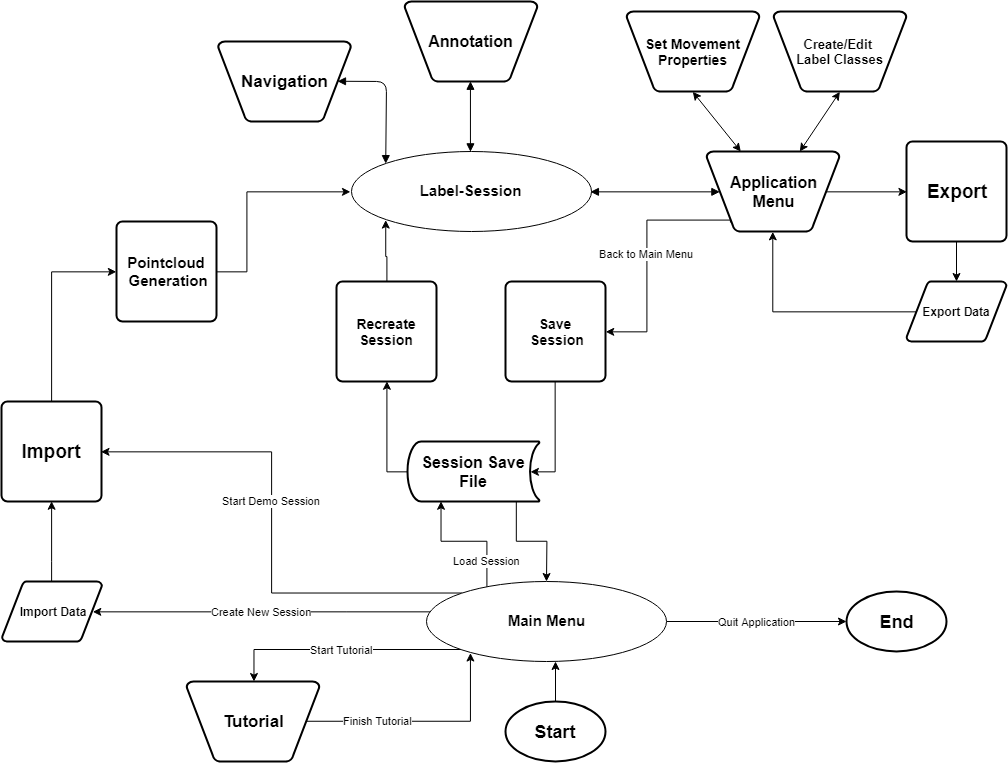
\includegraphics[width=15cm]{Workflow}
    \caption{\glslink{glos:Workflow} in C.LABEL-VR vom Import bis zum Export}
    \label{fig:Workflow}
\end{figure}


Der funktionelle Ablauf von C.LABEL-VR ist in der Abbildung \ref{fig:Workflow} grafisch dargestellt und wird in diesem Kapitel genauer erklärt. Nach dem Start der Applikation wird zunächst das Hauptmenü geladen (\textit{Main Menu}). Von dort aus gibt es mehrere Aktionsmöglichkeiten, die der Benutzer hat. Es kann eine Anleitung (\textit{Tutorial}) gestartet werden, in dem die Steuerung der Applikation erklärt wird. Nach Beendigung dieses Tutorials gelangt der Benutzer zurück ins Hauptmenü. Vom Hauptmenü aus kann die Applikation auch beendet werden. Zum Starten der Hauptapplikation gibt es drei Möglichkeiten. Mit Hauptapplikation ist eine \textit{Label-Session} gemeint, die aus mindestens einer Punktwolke besteht, welche visualisiert wird und annotiert werden kann. Der Benutzer kann zum einen eine Demonstrations-Session (\textit{Demo Session}) starten, bei der automatisch eine, von der Applikation zur Verfügung gestellte, Punktwolke geladen wird. Zum anderen kann eine neue Session gestartet werden. Dabei kann der Benutzer selbst auswählen, welche Dateien er einlesen möchte und von welchem Format diese sind. Die dritte Möglichkeit, wie eine Session gestartet werden kann, ist eine bestehende zu laden. Diese Möglichkeit besteht nur wenn es eine Speicherdatei zu einer Session gibt. Der Zeitpunkt der Erstellung einer solchen Datei wird im weiteren Verlauf dieses Kapitels genannt. \\

Startet der Benutzer eine neue, oder eine Demo-Session, werden die entsprechenden Dateien importiert und alle nötigen Informationen aus diesen extrahiert. Dieser Vorgang ist im Kapitel \ref{sec:ImportExport} genauer erläutert. Anschließend werden aus den extrahierten Informationen die Punktwolken für die Label-Session generiert. In Kapitel \ref{sec:Generierung} ist dieser Prozess beschrieben. Mit den Punktwolken kann nun eine Session gestartet werden. Möchte der Benutzer eine gespeicherte Session laden, so wählt er die entsprechende Speicherdatei aus. Aus dieser wird dann die Session wiederhergestellt.\\

Ist eine Label-Session nun gestartet, befindet sich der Benutzer innerhalb der virtuellen Punktwolke. Durch diese kann sich auf verschiedene Arten bewegt werden. Genaueres dazu ist in Kapitel \ref{sec:Navigation} zu finden. Neben der Navigation hat der Benutzer die Möglichkeit, die Punkte der Wolke zu annotieren. Auch hierzu gibt es mehrere Möglichkeiten, welche in Abschnitt \ref{sec:Annotation} beschrieben werden. Eine weitere Aktionsmöglichkeit, die es innerhalb einer Label-Session gibt, ist das öffnen eines Applikationsmenüs. In diesem Menü können Einstellungen im Bezug auf die Navigation festgelegt und geändert werden (\textit{Set Movement Properties}). Des Weiteren können Klassifikationen für die Annotation von Punkten erstellt oder bearbeitet werden (\textit{Create/Edit Label Classes}). Außerdem können, vom Applikationsmenü aus, die Daten, aus denen die Session durch den Import erstellt wurde, exportiert werden. In den Export fließen die Annotationen, welche der Benutzer während der Session getätigt hat, mit ein, sodass die exportierten Daten für weitere Anwendungsfälle, wie beispielsweise maschinelles Lernen (vgl. Kapitel \ref{sec:MLearning}) verwendet werden können.\\

Vom Applikationsmenü aus hat der Benutzer die Möglichkeit, zum Hauptmenü zurückzugelangen. Dabei wird die aktuelle Session gespeichert, sodass diese zu einem späteren Zeitpunkt weiter bearbeitet werden kann. Im Hauptmenü kann der Benutzer dann wieder eine neue Session starten, dass Tutorial ausführen, oder die Applikation beenden.


\section{Import und Export von Daten}
\label{sec:ImportExport}
Umfeldmodelle, welche in Form einer Punktwolke vorliegen, werden meist von einem Radar-, oder, wie in Kapitel \ref{sec:Lidar} gezeigt, von einem LiDAR-Sensor aufgenommen. Die Informationen über diese Modelle, zum Beispiel die Positionen der einzelnen Punkte, werden in einem passenden Datenformat abgespeichert. Um welches Format es sich dabei handelt, kann sehr unterschiedlich sein. In der Regel hängt es davon ab, zu welchem Zweck die aufgenommenen Daten gebraucht werden und wie umfangreich diese Daten sind. Am häufigsten werden sie dafür verwendet, um Lernalgorithmen und neuronale Netze (siehe Abschnitt \ref{sec:KNN}) zu trainieren. Automobilhersteller haben für solche Vorhaben unterschiedliche Konzepte und somit können auch die Formate der Daten unterschiedlich sein. Um die Applikation C.LABEL-VR für mehrere dieser Hersteller benutzbar zu machen, muss das Programm also mit verschiedenen Datenformaten umgehen können.\\ 

Innerhalb dieser Arbeit wurden mit zwei verschiedenen Arten von Daten gearbeitet. Das erste Format ist das PCD-Format (\textit{Point Cloud Data}). Die Bibliothek PCL (\textit{Point Cloud Library}) benutzt das Datenformat PCD, um Informationen über Punktwolken zu verwalten. PCL ist eine sehr mächtige C++-Bibliothek, die in der Regel von jedem benutzt wird, der performante Algorithmen für Punktwolken entwickeln möchte. Auch C.LABEL generiert aus eingelesenen Daten PCD-Files um Funktionen der Point Cloud Library für die Wolken zu benutzen.\\

Das zweite Format ist das, von der HDF-Group bereitgestellte, HDF5-Format (\textit{Heterogeneous Data Format}). Es ist ausgelegt zum schnellen Erstellen und Auslesen von komplexen und großen Datenstrukturen. Welche Elemente diese Strukturen enthalten können wird später in Kapitel \ref{sec:HDF5} erklärt. Zur schnellen Bearbeitung großer Datenmengen ist dies ein gängiges Format und wird von den meisten Kunden von CMORE benutzt um Sensordaten zu verwalten. Deshalb wird es auch in C.LABEL-VR verwendet.\\

Im folgenden Kapitel \ref{sec:Architecture} wird die Architektur des Import- und Export-Prozesses erläutert. Anschließend wird eine interne Datenstruktur in Abschnitt \ref{sec:IDS} vorgestellt, die aus Informationen besteht, die während des Import-Prozesses gesammelt wurden. Anschließend wird in Kapitel \ref{sec:HDF5} der gesamte Import und Export anhand eines Beispiels mit einer HDF5-Datei erklärt.

\subsection{Architektur}
\label{sec:Architecture}

Wichtig ist es also sowohl den Import, als auch den Export so modular wie möglich zu gestalten, dass C.LABEL-VR ohne große Änderungen  an der Hauptapplikation um neue Datenformate erweitert werden kann. Das Prinzip, das dafür entwickelt wurde, ist in Abbildung \ref{fig:ImportExport} dargestellt und wird im Folgenden näher erläutert. Die angesprochenen Erweiterungen um neue Datenformate werden als \textit{Addons} bezeichnet. Jedoch handelt es sich dabei nicht immer nur um eine Erweiterung eines, von Grund auf, neuen Datenformates. 
Bei Komplexen Datenformaten wie HDF5 kann der Entwickler die interne Struktur der Datei selbst bestimmen. Jede unterschiedliche Struktur muss auf unterschiedliche Weise eingelesen werden und braucht somit unterschiedliche Addons. Um die Erweiterbarkeit der Applikation sicherzustellen wurde der Import und der Export von der Hauptapplikation abgekapselt.

Dafür wurde eine interne Datenstruktur (kurz \acrshort{acr:IDS}) eingeführt, welche alle nötigen Informationen enthält, die für das \glslink{glos:Labeling}{Labeling} notwendig sind. Sie wird im späteren Kapitel \ref{sec:IDS} genauer vorgestellt. Der Vorteil dabei ist, dass die Hauptapplikation dadurch stets auf die gleiche Datenstruktur zurückgreifen kann. Sie bleibt somit unabhängig vom importierten Datenformat. Wird ein neues Import-Format eingeführt muss an der Hauptapplikation also nichts verändert werden. In der Abbildung \ref{fig:ImportExport} erkennt man, wie die Hauptapplikation (\textit{C.LABEL-VR Session}) nur mit internen Daten arbeitet und somit von den Import- und Exportdaten getrennt ist.\\ 

Jedes Import-Addon hat also zunächst die Aufgabe, seine jeweiligen Daten einzulesen und alle Informationen, die für die \acrshort{acr:IDS} notwendig sind, daraus zu extrahieren. Aus diesen Informationen können anschließend die entsprechenden Punktwolken generiert werden. Die Generierung wird in Kapitel \ref{sec:Generierung} erklärt. Beim Export ist es notwendig, dass die Struktur der Daten gleich bleibt, die vom Import-Addon eingelesenen wurden. Es sollen lediglich die \glslink{glos:Labeling}{Labeling}-Informationen aus der \acrshort{acr:IDS} hinzu- bzw. eingefügt werden. Aus der \acrshort{acr:IDS} kann das Export-Addon diese Informationen extrahieren und anschließend in die eingelesenen Daten exportieren. Die importierten Daten werden so allerdings überschrieben. Möchte man die Daten nicht überschreiben, müssen die Daten neu erstellt und mit den \glslink{glos:Labeling}{Labeling}-Informationen versehen werden. \\

Die Importierten Daten, beispielsweise HDF5, enthalten allerdings oft deutlich mehr Informationen, als für die interne Struktur notwendig. Diese Zusatzinformationen werden \textit{Metadaten} genannt. Für den Export bedeutet dies, dass man aus der internen Datenstruktur von C.LABEL-VR, die Struktur der anfangs eingelesenen Daten nicht wieder rekonstruieren kann, da die \textit{Metadaten} fehlen würden. Um dieses Problem zu lösen müssen die zusätzlichen Daten separat gespeichert werden. Dazu wurde eine erweiterbare Datenstruktur angelegt. In dieser kann man für jede Import-Struktur eine Metadatenstruktur anlegen. Das entsprechende Export-Addon kann die Metadaten dann verwenden um, zusammen mit den internen Daten, das gewünschte Exportformat zu rekonstruieren. \\

\begin{figure}%
	\centering
    \includegraphics[width=15cm]{Import_Export_Architecture}
    \caption{Das Import-Export-Prinzip in C.LABEL-VR}
    \label{fig:ImportExport}
\end{figure}

Zusammenfassend ist also folgendes zu tun, um die Benutzung ein neues Datenformates oder einer neuen Datenstruktur zu gewährleisten: Zunächst muss eine Importfunktion programmiert werden, die alle Informationen aus den gewünschten Daten ausliest. Anschließend muss diese Funktion das genormte, interne Datenformat (Kapitel \ref{sec:IDS}) erstellen und alle nötigen Informationen aus den eingelesenen Daten darin speichern. Daraus können die entsprechenden Punktwolken dann generiert werden. Falls es Daten gibt, die über diejenigen in der \acrshort{acr:IDS} hinausgehen, muss eine Metadatenstruktur angelegt werden, in welche die zusätzlichen Daten abgelegt werden können. Zuletzt ist eine Exportfunktion zu implementieren, welche die \glslink{glos:Labeling}{Labeling}-Informationen aus der internen Datenstruktur in die eingelesenen Daten exportieren kann. Außerdem muss sie in der Lage sein aus den internen- und den Metadaten das Ausgangsdatenformat wiederherzustellen, um die Daten als neue Files exportieren zu können. Im folgenden Kapitel soll dieses Prinzip konkret an einem HDF5-Beispiel gezeigt werden.

\subsection{Interne Datenstruktur}
\label{sec:IDS}
Wie im Kapitel \ref{sec:ImportExport} schon erwähnt, ist die interne Datenstruktur (\textit{IDS}) dafür da, um den Prozess des Imports und Exports von der Hautapplikation zu trennen. Dazu müssen aus den Daten die eingelesen werden sollen, alle Informationen extrahiert werden die für die interne Datenstruktur notwendig sind. Die IDS wird repräsentiert durch ein Skript, dass einem Objekt in Unity angehängt werden kann, also einer Komponente (vgl. Abschnitt \ref{sec:UnityDevelopment}). Jedem Punkt einer Wolke in C.LABEL-VR ist solch ein Skript zugeordnet. Das heißt aus jeder Punktinformation aus den Input-Daten wird ein IDS-Komponente erstellt. Eine solche Komponente besteht aus folgenden Eigenschaften:

\begin{itemize}
\item \textbf{ID}: Identifikationsnummer zur eindeutigen Erkennung des Punktes
\item \textbf{Label}: Information, zu welcher Klassifikation der Punkt gehört
\item \textbf{Position}: Dreidimensionale Position des Punktes
\item \textbf{Ground Point}: Information, ob der Punkt ein Bodenpunkt ist oder nicht
\end{itemize}

Dadurch kann die Möglichkeit genutzt werden, dass auf jede aktive Komponente eines Objekts in Unity zugegriffen werden kann. Wenn man nun beispielsweise einen Punkt identifiziert, den man neu klassifizieren möchte, kann auf die IDS-Komponente dieses Objekts zugegriffen werden und das darin enthaltene Label geändert werden.\\

Aus den Input-Daten wird meist nur die Position des Punktes ausgelesen und manchmal auch die Klassifikation des Punktes, falls diese schon vorhanden ist. Die ID wird innerhalb vom Import vergeben und dient dazu den Punkt eindeutig zu identifizieren. Werden beispielsweise Informationen eines Punktes als Metadaten abgespeichert, müssen diese später dem richtigen Punkt zugeordnet werden können. Dies geschieht über die eindeutige ID. Genauer erklärt wird dieser Vorgang im Abschnitt \ref{sec:HDF5Example}. Die Information, ob es sich um einen Bodenpunkt handelt oder nicht, wird nach dem Import von einem Algorithmus analysiert. Sie ist wichtig für die Cluster-Annotation, die später in Kapitel \ref{sec:ClusterLabeling} vorgestellt wird. Wie die Bodenpunkt-Analyse funktioniert wird in Abschnitt \ref{sec:GroundPointSegmentation} erklärt. \\

Da die interne Datenstruktur nicht viele Informationen enthält ist es eine simple Methode die Punktwolken-Daten in C.LABEL-VR zu verwalten. Alles was darüber hinaus geht kann in einer separaten Meta-Datei gespeichert werden, um die Zusatzinformationen beim Export zur Verfügung zu haben. Darüber hinaus ist sie leicht erweiterbar. Im Skript der IDS-Komponente müsste lediglich eine neue Eigenschaft angelegt werden, um jedem Punkt einer eingelesenen Punktwolke die neue Eigenschaft zuzuordnen. Das genaue Vorgehen bei der Bearbeitung der internen Datenstruktur und der Metadaten ist im folgenden Kapitel \ref{sec:HDF5Example} näher erklärt.

\subsection{HDF5}
\label{sec:HDF5}

HDF5 ist ein Datenformat, das von der \textit{HDF Group} entwickelt wurde und für das Abspeichern und Verwalten komplexer Datenstrukturen vorgesehen ist. Dazu bietet das Format eine Quellcode-Bibliothek und ein spezielles Datenmodell, das die Erstellung komplexer Datenstrukturen zulässt. HDF5 wurde entwickelt für die effiziente und schnelle Ein- und Ausgabe von großen und komplexen Daten \cite{bib:HDF5Main}. Des Weiteren wird eine hohe Flexibilität und Erweiterbarkeit des Datenformats geboten. Die Organisation des Formates ist im Folgenden erklärt.\\

HDF5-Daten sind in einer hierarchischen Struktur organisiert, die aus zwei primären Einzelstrukturen besteht. Diese zwei sind \textit{Groups} und \textit{Datasets}. Eine Group besteht aus einer beliebeigen Anzahl an HDF5-Strukturen. Sie kann also andere Groups oder Datasets enthalten. Zusätzlich können noch Metadaten, in Form von Attributen, in einer Gruppe gespeichert werden. Eine Group ist also vergleichbar mit einem Ordner in einem Windows-Betriebssystem. Datasets bestehen aus einer multidimensionalen Tabelle (\textit{Array}), in der Werte von verschiedenen Datentypen gespeichert werden können (\textit{Integer, Float, String,...}). Eine weitere Struktur ist die sogenannten \textit{Attribute}-Struktur. Sie ist eine verkleinerte Form eines Datasets und besteht in der Regel aus einem Namen und einem dazugehörigen Wert.\\

HDF5 wird in Bereichen wie beispielsweise Astronomie, Ingenieurwesen, Medizin oder Finanzwesen benutzt um große Datenmengen zu verwalten \cite{bib:WhoUsesHDF}. Auch in der Automobilbranche wird es benutzt, beispielsweise ist die Nachfrage für dieses Datenformat bei der CMORE Automotive GmbH groß. Deswegen wurde beim Import und Export von C.LABEL-VR großen Wert darauf gelegt, dass dieses Format mit der Applikation kompatibel ist. Im Folgenden wird der Import/Export-Prozess anhand eines HDF5-Beispiels erläutert, da dieses Format alle Funktionen des Import/Export-Prozesses in C.LABEL-VR nutzt.

\subsubsection{HDF5 Import/Export-Beispiel}
\label{sec:HDF5Example}

\begin{figure}%
    \centering
    \subfloat[Dataset mit Größe 1x10]{{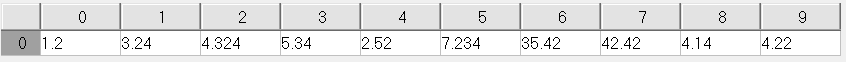
\includegraphics[width=14cm]{ExampleDataset}\label{fig:HDF5Dataset}}}%
    \qquad
    \subfloat[Aufbau der Beispiel HDF5-Datei]{{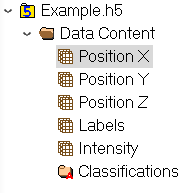
\includegraphics[width=4cm]{ExampleH5}\label{fig:HDF5Structure}}}%
    \qquad
    \subfloat[Attribute von \textit{Classifications}]{{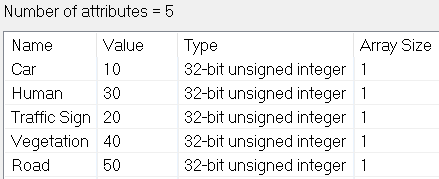
\includegraphics[width=9cm]{ExampleAttributes}\label{fig:HDF5Attributes}}}%
    \caption{Die Abbildungen zeigen Beispiele für die Inhalte einer HDF5-Datei}
\end{figure}

Für dieses Beispiel wird eine HDF5-Datei benutzt, welche Informationen über eine Punktwolke beinhaltet, die von einem LiDAR-Sensor (siehe Kapitel \ref{sec:Lidar}) aufgenommen wurde. Die Struktur der Datei besteht aus einer primären Group mit dem Namen \textit{Data Content}, die den Inhalt der einzelnen Daten (siehe Abbildung \ref{fig:HDF5Structure}). In dieser Group befinden sich fünf Datasets und eine Attribute-Struktur. Drei dieser Datasets definieren die Positionen der einzelnen Punkte der Wolke. Jedes dieser drei Positions-Datasets steht für den Wert, welchen die Punkte auf einer kartesischen Achse haben. Das heißt ein Dataset beinhaltet alle X-Koordinaten, ein anderes alle Y-Koordinaten und das dritte alle Z-Koordinaten der Punkte. Das vierte Dataset beinhaltet eine Tabelle, in der die Labels aller Punkte zu finden sind. Das letzte Dataset beinhaltet den Intensitätswert, mit dem der reflektierte Lichtimpuls zurück auf den Sensor getroffen ist. Die Attribut-Struktur besteht aus einer Spalte mit dem Namen des Attributs und einer zweiten Spalte mit dem dazugehörigen Attributswert. Zusätzlich ist bei jedem Attribut der Datentyp und die Größe der Datentabelle angegeben. Diese Attributs-Struktur repräsentiert eine vorgefertigte Anzahl an Klassifikationen, mit denen Punkte in C.LABEL-VR annotiert werden können.\\

\subsubsection{Import}

Die Quellcode-Bibliothek, die von der HDF Group zur Verfügung gestellt wird, bietet Funktionen zum Lesen und Schreiben von bzw. aus einer HDF5-Datei. Beim Lesen muss die Tabellengröße der zu lesenden Struktur bekannt sein. Bei einem Dataset, wie in Abbildung \ref{fig:HDF5Dataset}, muss eine Tabelle angelegt werden, die eine Zeile und 10 Spalten hat. In diese Tabelle kann dieses Dataset, mit Hilfe der Funktion aus der Quellcode-Bibliothek, importiert werden. Bei der Attributs-Struktur wird jedes Attribut einzeln ausgelesen, da die Struktur aller Attributwerte unterschiedlich sein kann. In Abbildung \ref{fig:HDF5Attributes} bestehen alle Werte (\textit{Values}) aus einer Zahl, da die Werte der Identifikationsnummer der Klassifikation entsprechen. Werte können aber auch aus unterschiedlich großen Tabellen bestehen. Deswegen muss jedes Attribut einzeln gelesen werden.\\

Sind alle Information ausgelesen, kann der Importprozess in C.LABEL-VR abgeschlossen werden. Dazu müssen alle Informationen richtig verteilt werden. Die Punktwolke aus der Beispieldatei besteht aus zehn Punkten, da in den Datasets eine Tabelle mit zehn Werten vorhanden ist (siehe Abbildung \ref{fig:HDF5Dataset}). Das bedeutet, dass zunächst zehn Dateien der internen Datenstruktur erstellt werden (vgl. Kapitel \ref{sec:IDS}). Jeder Datei wird nach der Reihe, aufsteigend eine ID von 0-9 zugeordnet, sodass jeder Punkt eine einmalige ID hat. Anschließend können die Werte aus den Datasets \textit{Position X}, \textit{Position Y} und \textit{Position Z} den Positionswerten der IDS zugeordnet werden. Die Werte aus dem Dataset \textit{Labels} werden der Label-Komponente der IDS zugeordnet. Die \textit{Ground Point}-Information ist nicht Inhalt der HDF5-Datei. Wie diese Information erlangt wird ist in Kapitel \ref{sec:GroundPointSegmentation} beschrieben.\\

In C.LABEL-VR ist es möglich die Punkte einer Punktwolke mit unterschiedlichen Klassifikationen zu annotieren. Dazu können Klassifikationen neu erstellt oder bearbeitet werden. Wie dies funktioniert und wie unter den Klassifikationen ausgewählt werden kann ist in Kapitel \ref{sec:Annotation} beschrieben. Die Klassifikationen, welche in der Attributsstruktur \textit{Classifications} zu finden sind (siehe Abbildung \ref{fig:HDF5Attributes}), können somit beim Import schon verwendet werden. Dazu werden diese Informationen in eine C\#{}-Klasse geschrieben, mit welcher C.LABEL-VR alle Informationen über Labels verwaltet. \\

Die Informationen des Datasets \textit{Intensity}, welches die Intensitätswerte enthält, mit denen die reflektierten Lichtimpulse zurück auf den Sensor getroffen sind, haben für die Applikation keine Relevanz. Deswegen werden sie in eine Tabelle innerhalb einer separaten C\#{}-Klasse gespeichert, in der die Applikation alle Metadaten verwaltet (vgl. \textit{HDF5 Meta Data} in Abbildung \ref{fig:ImportExport}). Zusätzlich muss in dieser Meta-Datei noch eine andere Information gespeichert werden. Die Werte aller Datasets dieser Beispieldatei sind an der jeweiligen Tabellenstelle einem jeweiligen Punkt zugehörig. Das bedeutet, dass alle Werte der Datasets, zum Beispiel an der Tabellenstelle (0,0), zu einem Punkt gehören. Deswegen müssen alle Werte stets an der richtigen Tabellenstelle sein. Um dies auch beim späteren Export zu gewährleisten wird eine Datenstruktur in der Meta-Datei erstellt, welche die ID jedes Punktes mit der Tabellenstelle verknüpft. Somit kann von jedem Punkt, einzeln die Information abgefragt werden, an welche Tabellenstelle in den Datasets die Werte des Punktes zugehörig sind.\\

Ist die Speicherung all dieser Informationen an der richtigen Stelle abgeschlossen, ist der Import beendet und es kann mit dem Beginn der Punktwolkengenerierung angefangen werden. Diese ist im folgenden Kapitel \ref{sec:Generierung} erläutert.


\subsubsection{Export}

Beim Export der HDF5-Datei müssen alle nötigen Informationen gesammelt werden, damit die Ausgansstruktur der Datei wiederhergestellt werden kann. Zunächst werden Tabellen, mit der richtigen Größe, für alle Datasets erstellt. In diesem Beispiel haben die Tabellen eine Zeile und zehn Spalten. In diese Tabellen können anschließend die entsprechenden Werte eingetragen werden. Dazu wird zunächst durch alle Punkte der Wolke iteriert und die Information über ID, Label und Position des Punktes abgefragt. Mit Hilfe der Zuweisungstabelle aus der Meta-Datei, kann anhand der ID herausgefunden werden, an welche Tabellenstelle die Positions- und Labelinformation des Punktes geschrieben werden muss. Somit kann jede Koordinate des Punktes an die richtige Stelle der entsprechenden Tabelle geschrieben werden und das Label des Punktes an die richtige Stelle der Label-Tabelle. Auf diese Weise ist das Label- und die Positions-Datasets wiederhergestellt. Die Tabelle mit den Intensitätswerten wird einfach aus der Meta-Datei kopiert, da diese Informationen nie einem Punkt zugewiesen wurden. Zuletzt werden die Klassifikationen aus der C\#{}-Label-Klasse gelesen und in eine entsprechende Tabelle geschrieben. \\

Sind alle Werte den Tabellen zugewiesen worden, kann eine neue HDF5-Datei erstellt werden, welche die gleichen Strukturen enthält, wie die eingelesene Datei. Das bedeutet es wird eine Group erstellt, welche sowohl fünf Datasets mit jeweils einer Zeile und 10 Spalten enthält, als auch einer Attributsstruktur. Die Tabellen mit den Positions-, Label- und Intensitätswerten, werden direkt in die entsprechenden Datasets geschrieben. Von der Liste aller Klassifikationen aus der C\#{}-Label-Klasse wird jeder Klassifikation mit dem jeweiligen Klassifikationswert einzeln in die Attributsstruktur geschrieben. Ist dieser Vorgang beendet, ist auch der Export der Datei beendet, da die Struktur dieser Datei vollständig wiederhergestellt wurde und der Inhalt der Datei aus der C.LABEL-VR-Applikation eingefügt wurde. 

\section{Generierung einer Punktwolke}
\label{sec:Generierung}
\begin{figure}%
    \centering
    \subfloat[C.Label]{\fbox{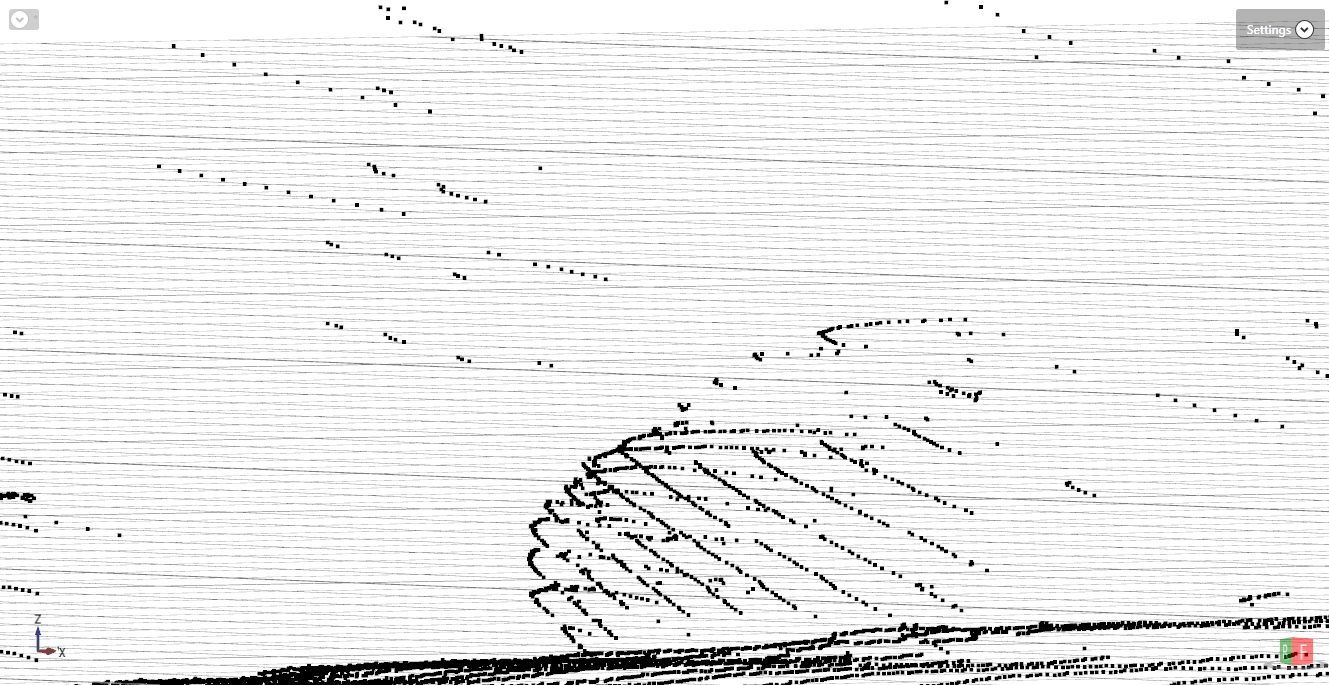
\includegraphics[width=7cm]{CarClabel}\label{fig:CarClabel}}}%
    \quad
    \subfloat[C.Label-VR]{\fbox{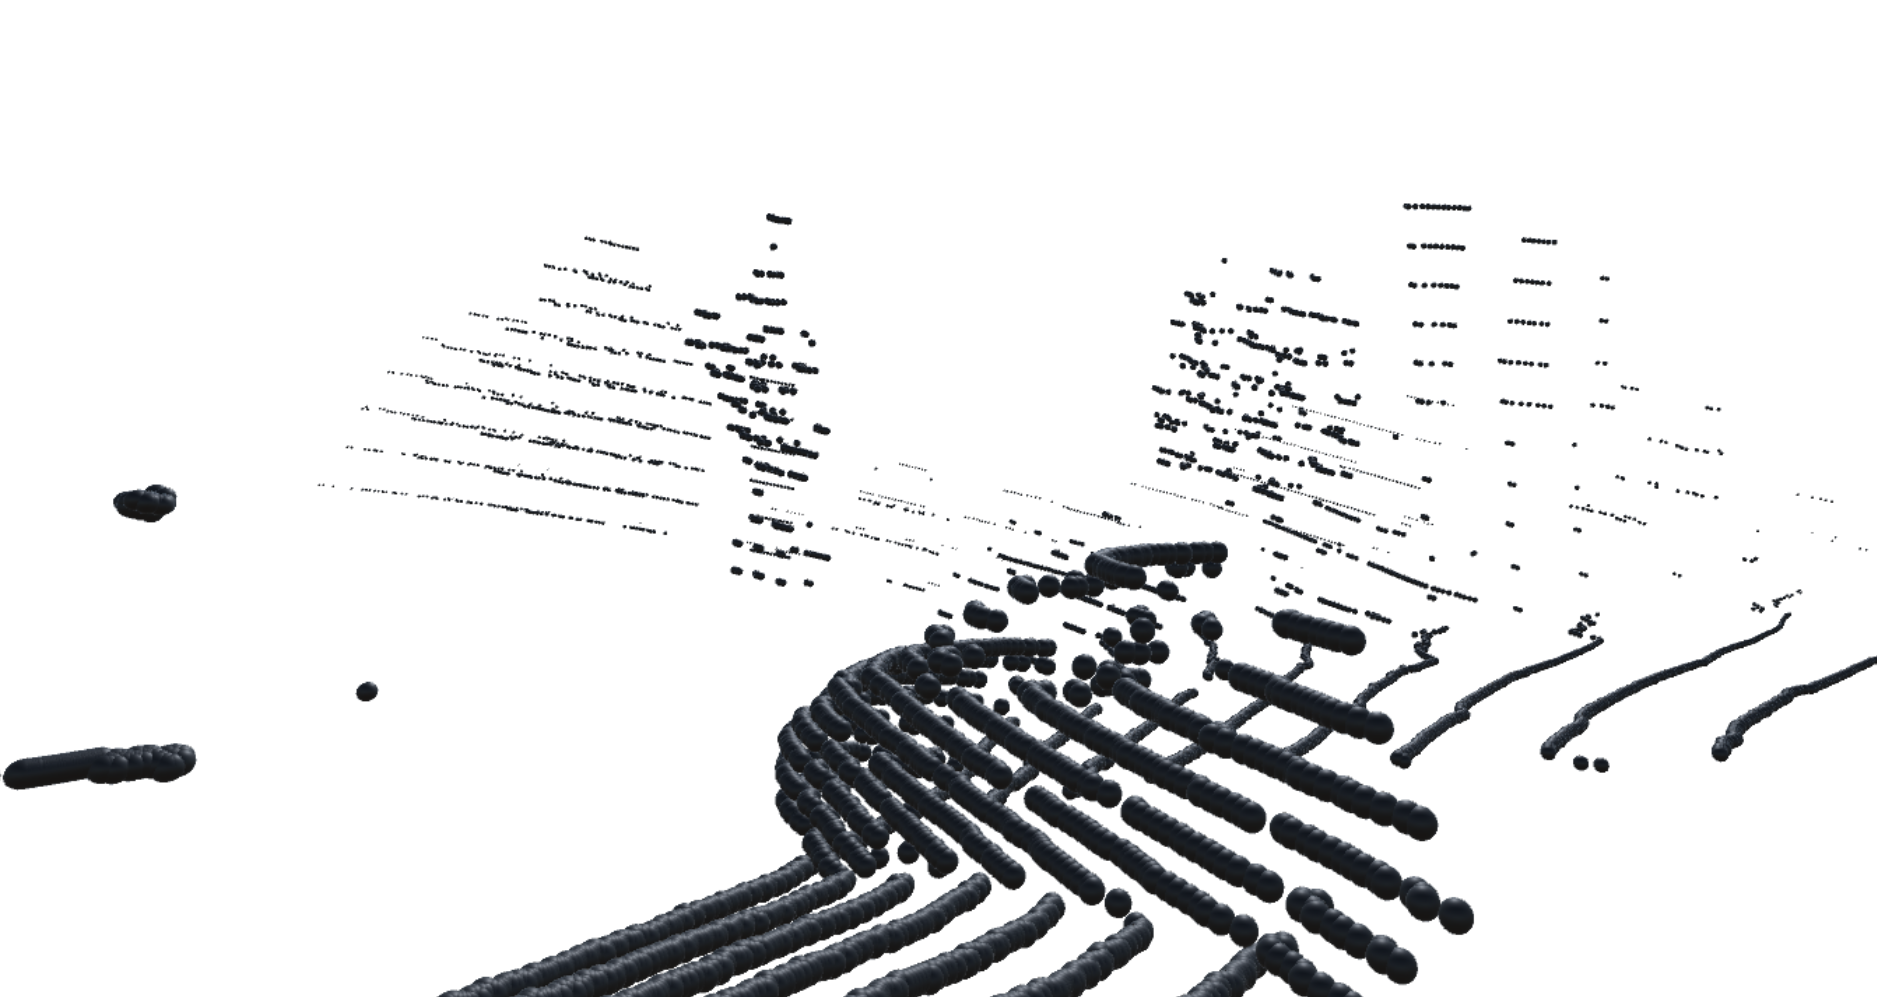
\includegraphics[width=6.8cm]{CarClabelVR}\label{fig:CarClabelVR}}}%
    \caption{Vergleich der Darstellung von Perspektive und Tiefe zwischen C.LABEL und C.LABEL-VR}
    \label{fig:CloudCompare}%
\end{figure}

Nach dem man die Informationen über die internen Datenstrukturen durch den Import gesammelt hat, kann man mit der Generierung der Punktwolken anfangen. Ziel davon ist es die Punktwolkendaten zu visualisieren, damit der Benutzer sie sehen und mit ihnen interagieren kann. In der Regel wird dafür, in einer passenden Visualisierungsumgebung, für jede Position eines Punktes ein Objekt eingezeichnet. Meistens sind dies zweidimensionale Punkte, die lediglich eine quadratische Einfärbung von Pixeln sind (siehe Abbildung \ref{fig:CarClabel}).\\

In C.Label-VR wird jeder Punkt durch eine dreidimensionale Kugel repräsentiert (siehe Abbildung \ref{fig:CarClabelVR}). Dadurch wird für den Benutzer der Eindruck erzeugt, dass die Sensordaten durch echte Objekte im Raum repräsentiert werden. Diese Objekte, sind durch ihre dreidimensionale Eigenschaft gut sichtbar sind und wirken für den Benutzer greifbar. Dies ist ein großer Unterschied zu bisherigen Visualisierungen und bietet einen erheblichen optischen Mehrwert. Die Unity Engine, als Visualisierungsumgebung, bietet nämlich die richtige Darstellung der räumlichen Proportionen an jeder Position. Diese Proportionen, also auch die Darstellung der Sensordaten im richtigen Maßstab, werden durch das Rendering der Unity Engine für jedes Bild berechnet (erklärt in Abschnitt \ref{sec:UnityDevelopment}) und somit immer richtig für den Benutzer dargestellt.\\

Die dreidimensionalen Punkte sind dabei vorgefertigte Objekte. Dieses Vorfertigen von Objekten bietet sich bei der Entwicklung mit Unity immer dann an, wenn mehrere gleiche Objekte zur gleichen Zeit existieren sollen, wie es beispielsweise bei einer Punktwolke der Fall ist. Die Erstellung solcher Objekte, die in Unity \textit{Prefabs} genannt werden, ist eine herkömmliche Methode bei der Entwicklung mit Unity \cite{bib:UnityPrefab}.\\ 

\begin{figure}%
    \centering
    \subfloat[Mesh Filter- und Collider-Komponente]{{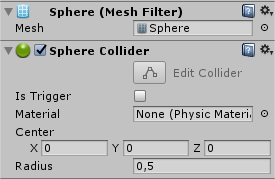
\includegraphics[width=8cm, height=5.5cm]{ComponentMeshCollider}\label{fig:MeshCollider}}}%
    \qquad
    \subfloat[Mesh Renderer-Komponente]{{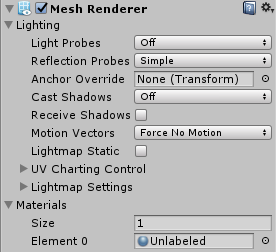
\includegraphics[width=6cm, height=5.5cm]{ComponentMeshRenderer}\label{fig:MeshRenderer}}}%
    \caption{Beide Bilder zeigen Komponenten aus der Unity Editor, die dem Punkt-Prefab zugeordnet sind.}
    \label{fig:Components}%
\end{figure}

Das Punkt-Prefab, das für C.LABEL-VR vorgefertigt wurde um einen Punkt in der Punktwolke zu repräsentieren, besteht dabei aus mehreren Komponenten. Eine Komponente ist dabei die Transform-Komponente (siehe Abschnitt \ref{sec:UnityDevelopment}), welche die Position des Punktes festlegt. Eine weitere ist die \textit{Mesh Renderer}-Komponente. Ein Mesh (zu deutsch: Gewebe/Netz) ist in der Spielentwicklung ein gängiger Begriff für das dreidimensionale Modell eines Objektes \cite{bib:Meshes}. Für das Punkt-Prefab wird das Modell einer Kugel verwendet (\textit{Sphere} als Mesh in Abbildung \ref{fig:MeshCollider}). Der Mesh-Renderer legt dabei die Materialeigenschaften des Objektes fest \cite{bib:MeshRenderer}. Diese Eigenschaften enthalten beispielsweise die Textur, also das Aussehen der Oberfläche des Objektes, die Reflexionseigenschaften oder wie die Art wie das Objekt Lichteinwirkungen auf die Umgebung verteilt. Das Standard-Material das beim Punkt-Prefab verwendet wird ist ein vorgefertigtes Material \textit{Unlabeled} (siehe Abbildung \ref{fig:MeshRenderer}), welches eine einfarbige, schwarze Oberfläche hat. Schwarze Punkte repräsentieren also diejenigen Punkte, die noch nicht annotiert wurden. Andere Eigenschaften wie Licht, Reflexionen oder Schatten wurden mit Parametern belegt, die so wenig wie möglich Berechnungen erfordern, damit die Bildwiederholungsrate der Applikation so hoch wie möglich gehalten werden kann. Genauer ist dies im folgenden Abschnitt \ref{sec:Optimierung} erklärt. \\

Eine weitere wichtige Komponente ist der \textit{Sphere Collider} (siehe Abbildung \ref{fig:MeshCollider}). Sie ist notwendig um mit dem Punkt zu interagieren, da der Sphere Collider die Kollisionseigenschaften des Objektes festlegt. Möchte man mit dem Punkt beispielsweise durch einen anderen virtuellen Gegenstand interagieren, muss die Kollision zwischen Punkt und dem Gegenstand detektiert werden. Dazu ist die Collider-Komponente bei einem Kollisionsobjekt notwendig. Wie des Detektion genau funktioniert ist im späteren Kapitel \ref{sec:SimplePointerAnnotation} beschrieben, in dem es um die Interaktion mit Punkten geht. Ebenfalls wichtig für die Leistungsfähigkeit von C.LABEL-VR ist es, dass die \textit{Is Trigger}-Eigenschaft des Punkt-Colliders deaktiviert ist. Im aktiven Zustand besagt diese Eigenschaft, dass das Objekt welches diesen Collider hat, der Auslöser für Kollisionen ist. Das heißt die Collider-Komponente überprüft durchgehend ob eine Kollision vorliegt. Wenn alle Punkte der Wolke diese Überprüfung durchgehen machen würden, würde sich das negativ auf die Leistung der Applikation auswirken.\\

Zuletzt enthält das Punkt-Prefab doch die Komponente der internen Datenstruktur (vgl. Abschnitt \ref{sec:IDS}). Diese enthält die Informationen die man bei der Interaktion mit dem Punkt wissen muss, wie das Label und die Position. Die Label-Eigenschaft der IDS-Komponente wurde so implementiert, dass sie mit der Mesh-Renderer Komponente verknüpft ist. Dies dient dem Zweck, dass sich bei Änderung des Labels automatisch die Material-Farbe des Punktes ändert. Eine ähnliche Verknüpfung gibt es bei der Positionseigenschaft der internen Datenstruktur. Diese ist mit der Transform-Komponente verknüpft, sodass bei Änderung der Positionseigenschaft auch wirklich die Position geändert wird, da dies nur mit der Transform-Komponente möglich ist. Beide Implementationen sind in der Auflistung \ref{lst:ComponentConnection} zu sehen.

\begin{lstlisting}[caption={Verknupfung von Label- und Positionseigenschaft der IDS-Komponente mit anderen Komponenten}, captionpos=t,numbers=left , label=lst:ComponentConnection]
private uint _Label;
public uint Label
{
    get
    {
        return _Label;
    }
    set
    {
        _Label = value;
        GetComponent<MeshRenderer>().material = 
        	Labeling.GetLabelClassMaterial(_Label);
    }
}

private Vector3 _PointPosition;
public Vector3 PointPosition
{
    get
    {
        return transform.position;
    }
    set
    {
        transform.position = value;
    }
}
\end{lstlisting}
\quad

\begin{figure}%
	\centering
    \fbox{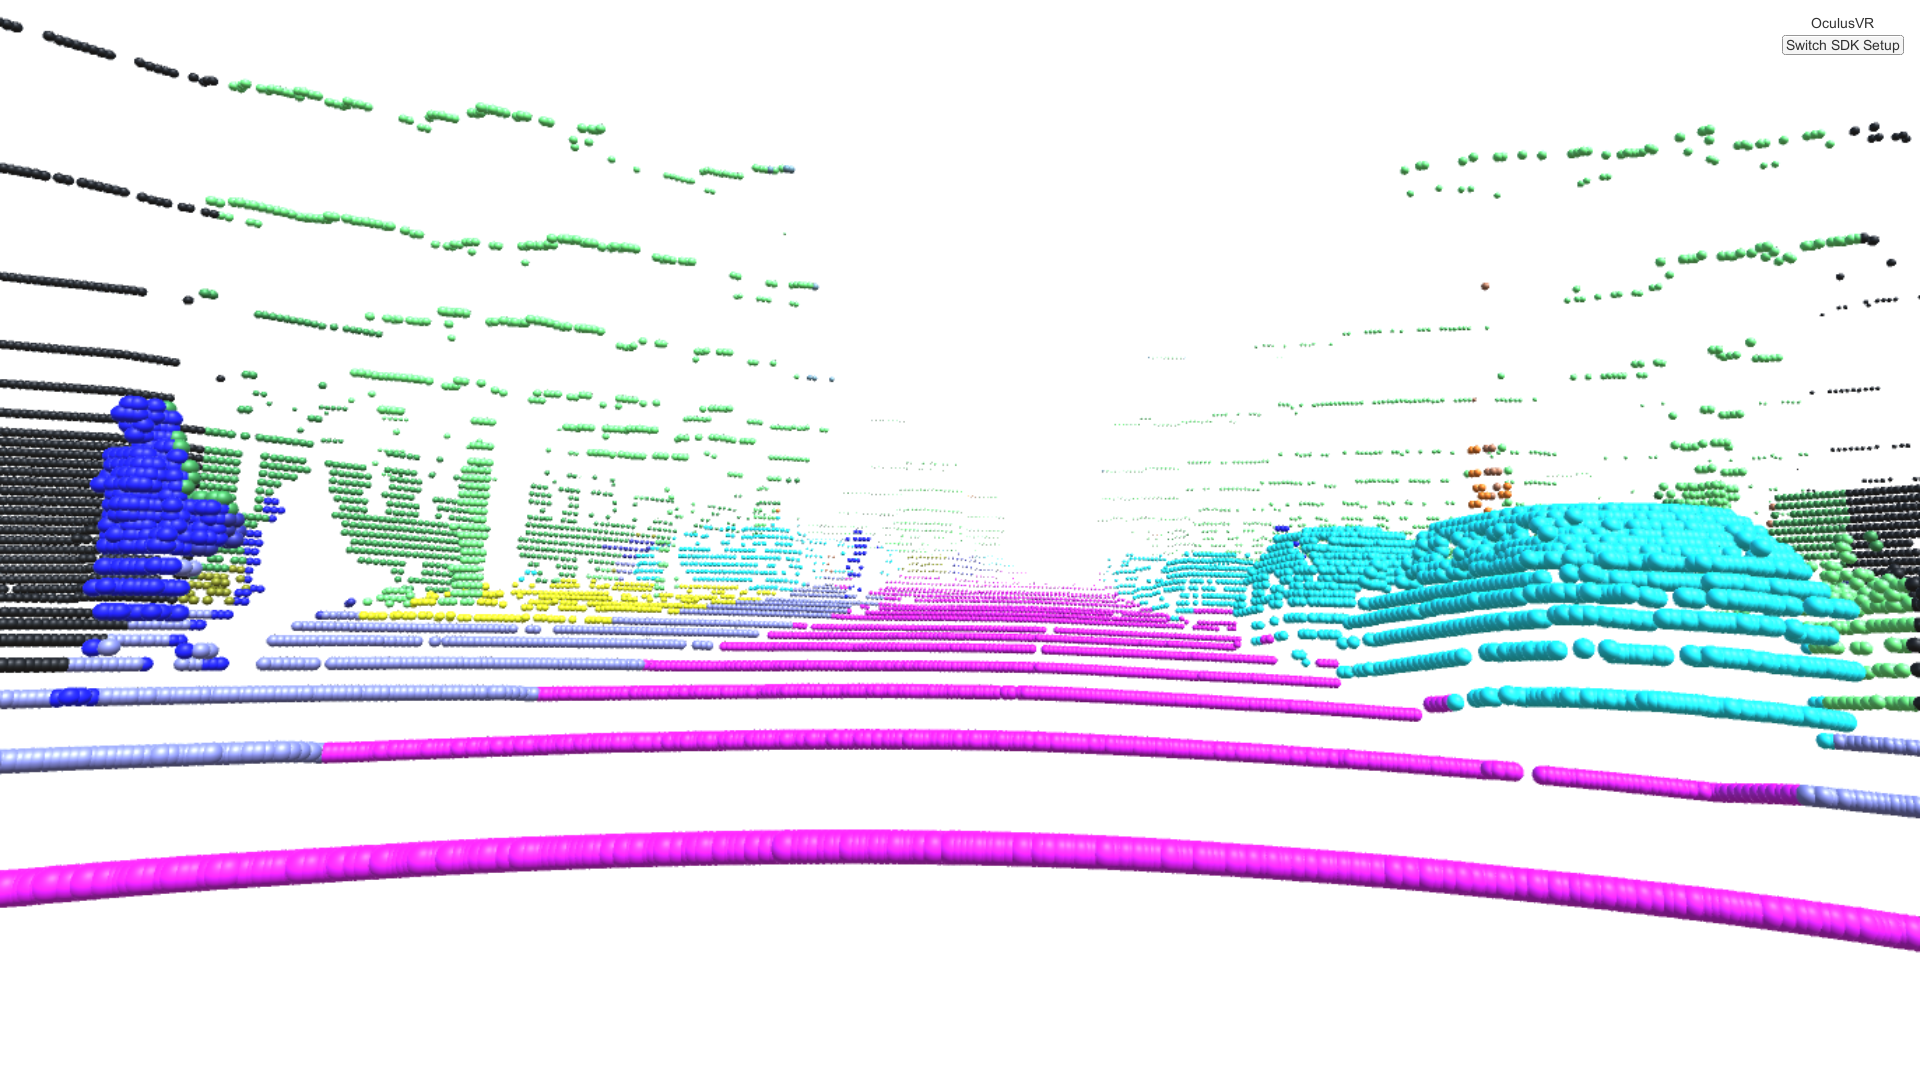
\includegraphics[width=15cm]{PreLabeledPointcloud}}
    \caption{Punktwolke in C.LABEL-VR mit mit Annotationen, die beim Einlesen der Daten schon vorhanden sind.}
    \label{fig:PreLabelCloud}
\end{figure}

Das Punkt-Prefab, mit all seinen Komponenten und deren richtig festgelegten Eigenschaften, kann nun für jeden Punkt aus den Input-Daten instantiiert werden. Dafür gitb es in Unity die spezielle Funktion \textit{Instantiate} \cite{bib:Instantiate}. Die Unity Engine klont dadurch für jede Instanz das vorgefertigte Ausgangsobjekt, wobei jedes der Klone nach der Instantiierung individuell veränderbar ist. Nachdem die Instanz eines Punktes erstellt wurde kann also seine Position festgelegt werden und, wenn beim Import schon vorhanden, das Label des Punktes gesetzt werden (vgl. Abbildung \ref{fig:PreLabelCloud}). Durch das Vorgehen, das in diesem Abschnitt beschrieben wurde entsteht eine Punktwolke, welche in einer virtuellen Umgebung betrachtet werden kann. 

\subsection{Optimierung der Bildwiederholungsrate}
\label{sec:Optimierung}

Die Bildwiederholungsrate einer Applikation ist wesentlich entscheidend für die Benutzererfahrung mit ihr. Geringe Wiederholungsraten führen zu einer nicht flüssigen Darstellung des Applikationsinhaltes, was sehr störend für den Benutzer sein kann. Gerade bei VR-Apllikationen sind konstant hohe Bildwiederholungsraten wichtig um dem Benutzer eine angenehme visuelle Präsentation zu bieten und keine Symptome der VR-Krankheit hervorzurufen. Nähere Informationen zur VR-Krankheit werden im folgenden Abschnitt \ref{sec:VRSickness} gegeben. In C.LABEL-VR werden keine komplexen 3D-Objekte oder hochauflösende Texturen dargestellt, deswegen könnte hier der Eindruck entstehen, dass die Applikation, bei einem Leistungsstarken Rechner wie in Abschnitt \ref{sec:VR-Rechner}, keine Performance-Probleme haben sollte. Da aber Punktwolkendaten oft über 30.000 Punkte enthalten können, ist die große Anzahl an Objekten selbst, die dargestellt werden muss, auch für leistungsstarke Rechenmaschinen eine Herausforderung. Deswegen muss bei der Erstellung der Punktwolken auf einige Dinge geachtet werden, um keine Einbrüche bei der Bildwiederholungsrate zu verursachen.\\

Im Abschnitt \ref{sec:UnityDevelopment} wurde die Update-Funktion erwähnt, die bei jedem Bildwiederholungszyklus in Unity ausgeführt wird. Durch diese hohe Ausführungsrate ist es generell ratsam, so wenig wie möglich Leistungsintesiven Programm-Code in diesen Methoden zu verwenden, da dieser ständig ausgeführt wird. Bei der Erstellung von Punktwolken in C.LABEL-VR ist es außerdem wichtig, dass das Punkt-Prefab über keine dieser Update Methoden verfügt. Diese würde nämlich von allen Punkten durchgehend ausgeführt werden, was bei einer hohen Anzahl an Punkten zu einem großen Leistungsverlust führen würde.\\

Wichtig bei der Erstellung des vorgefertigten Punktes ist es auch, die Materialeigenschaften richtig zu wählen. Das Material selbst, das dem Punkt-Prefab zugeordnet ist, ist ebenfalls vorgefertigt (Material \textit{Unlabeled} in Abbildung \ref{fig:MeshRenderer}). Der Unity Engine ist somit bekannt, dass jeder darzustellende Punkt das gleiche Material hat. Die Engine muss somit nicht für jeden neuen Punkt eine neue Information über das Material anfordern. Vergleichbar ist dieser Vorgang mit dem Bohren eines Loches. Ist die Größe des Loches bekanntermaßen immer gleich, so muss der Bohrkopf nie gewechselt werden. Das spart Zeit und schlägt sich in C.LABEL-VR durch weniger Berechnungszeit und damit eine höhere Bildwiederholungsrate nieder.\\

Bei den Eigenschaften der Mesh Renderer-Komponente (siehe Abbildung \ref{fig:MeshRenderer}) kann ebenfalls darauf geachtet werden, keine unnötigen Berechnungen zuzulassen. Die Optionen \textit{Light Probes} und \textit{Lightmap Static} sind für die Lichtverteilung des Objektes in der Szene zuständig \cite{bib:LightProbes}. Da eine Lichtverteilung des Objektes keinen optischen Mehrwert bringt, da der Hintergrund weiß ist, können diese Optionen deaktiviert werden um Rechenzeit zu sparen. Auch die Option \textit{Cast Shadows} wird deaktiviert, da das Anzeigen von Schatten bei der Berechnung aufwendig und bei der Darstellung der Punktwolke nicht erwünscht ist. Lediglich die Eigenschaft \textit{Reflection Probes} wird mit der Option \textit{Simple} belegt. Diese Eigenschaft legt die Reflexion, die vom Objekt zurückgegeben wird fest. Solch eine Reflexion ist in C.LABEL-VR gewünscht, da dies die Punkte für den Benutzer räumlicher darstellt, da sie Reflexionen wie echte Objekte haben. Damit die Berechnungen dafür aber nicht zu aufwendig werden, wird hier nur die Option Simple gewählt.\\

Auch bei der Sphere Collider-Komponente ist auf eine Eigenschaft zu achten. Wie schon in Abschnitt \ref{sec:Generierung} erwähnt, ist diese Komponente für die Interaktion mit dem Objekt zuständig. Durch diese Komponente kann nämlich detektiert werden, ob  es eine Kollision mit einem anderen Objekt gibt, welches ebenfalls einen Collider besitzt \cite{bib:Collider}. Eine der beiden Collider-Komponenten muss dabei der Auslöser der Kollision sein. Um dies zu gewährleisten kann die Eigenschaft \textit{Is Trigger} aktiviert werden (siehe Abbildung \ref{fig:MeshCollider}). Ist diese im aktiven Zustand, so überprüft die Collider-Komponente durchgehend, ob eine Kollision mit einem anderen Objekt vorliegt. Ist dies bei jedem Punkt in der Punktwolke der Fall, gibt es durchgehend von allen Punkten diese Überprüfung, was zu einem erheblichen Performance-Verlust führt. Möchte man also durch ein Objekt mit einem Punkt interagieren, muss das Objekt der Auslöser der Kollision sein. Somit gibt es nur ein Objekt in der Szene, welches eine Kollisionsprüfung vollzieht.\\

Trotz all dieser Einstellungen zur Verbesserung der Anwendungs-Performance kann es bei zu vielen Punkten im Sichtfeld des Benutzers zu einer niedrigen Bildwiederholungsrate kommen. Der Grund dafür ist, dass für jedes anzuzeigende Objekt ein Zeichnungs-Befehl an die Grafikkomponente des Rechners gegeben werden muss. Dies wird in der Fachsprache \textit{Draw Call} genannt \cite{bib:DrawCall}. Bei einer zu hohen Anzahl an Punkten in einer Punktwolke, kann es somit zu einer zu hohen Anzahl an Zeichnungs-Befehlen kommen. Dies führt dann zu einer niedrigen Bildwiederholungsrate. In diesem Fall hilft die Verbesserung der Leistungskomponenten des VR-Rechners (vgl. Abschnitt \ref{sec:VR-Rechner}). Für C.LABEL-VR wurde als zusätzliche Leistungsoptimierung eine Funktion implementiert, die dieses Problem umgeht. Diese Funktion verringert die Anzahl der angezeigten Punkte während der Bewegung des Benutzers, um die Anzahl an Draw-Calls zu verringern und somit die Bildwiederholungsrate zu erhöhen. Diese Funktion wird näher im Abschnitt \ref{sec:AppMenu} erklärt. 

\section{Navigation}
\label{sec:Navigation}
Die Navigigation in Virtual Reality-Anwendungen ist ein entscheidendes Thema. Wird dieses Thema während der Entwicklung einer VR-Applikation nicht ausreichend berücksichtigt, so kann dies große Auswirkung auf die Benutzererfahrung haben \cite{bib:PointTeleport}. Ein Grund dafür ist die \textit{VR-Krankheit}, die häufig auftritt wenn sich Benutzer durch eine virtuelle Umgebung bewegen \cite{bib:VRSicknessLaviola}. Diese Krankheit verursacht unter anderem Übelkeit und tritt bei manchen Nutzern mehr und bei manchen weniger auf. Details dazu sind im Abschnitt \ref{sec:VRSickness} gegeben. \\

Um sich in C.LABEL durch Punktwolken zu Bewegen wurden zwei Navigationsmöglichkeiten entwickelt. Zum einen gibt es den Freien Flug Modus (Abschnitt \ref{sec:FreeFlyMode}). In diesem Modus kann sich der Benutzer, mit Hilfe der Oculus Eingabegeräte intuitiv und frei durch die Punktwolke bewegen. Die Bewegung ist dabei durchgängig und wird durch Beschleunigung und Bremsen gestartet und beendet. Diese Art der Bewegung fördert jedoch bei manchen Nutzen den Effekt der VR-Krankheit.\\

Deshalb gibt es mit dem Teleportationsmodus (\textit{Teleport Mode}) noch eine alternative Navigationsart (\ref{sec:TeleportMode}). Das Grundprinzip der Steuerung ist ähnlich, allerdings gibt es keine durchgängige Bewegung. Stattdessen wird der Benutzer von einer Stelle zur anderen teleportiert. Dies wirkt dem Übelkeitseffekt entgegen.   

\subsection{VR-Krankheit}
\label{sec:VRSickness}
Die VR-Krankheit ist ein Effekt der auftritt während oder nach dem Aufenthalt einer Person in einer virtuellen Umgebung. Sie äußert sich meistens durch Übelkeit, aber auch durch andere Symptome wie Kopfschmerzen oder Überanstrengung der Augen \cite{bib:VRSicknessLaviola}. Es wird geschätzt, dass bei dreißig bis achtzig Prozent der Menschen Symptome der VR-Krankheit auftreten wenn sie sich in einer virtuellen Umgebung befinden \cite{bib:VRSicknessRebenitsch}. Die Erforschung der Ursache für diese Krankheit ist noch nicht gänzlich abgeschlossen. Somit gibt es mehrere Theorien was der Auslöser für sie ist.\\

Die gängigste Theorie dafür ist das Prinzip der Sinnestäuschung. Dieses Prinzip besagt, dass das menschliche Gehirn einen Konflikt feststellt, wenn sich die erwartete Wahrnehmung zweier Sinnesorgane voneinander unterscheiden. Im Falle der VR-Krankheit handelt es sich bei den Sinnesorganen um die visuelle Wahrnehmung und den Gleichgewichtssinn. Bewegt sich ein VR-Nutzer nun durch die virtuelle Welt, so registriert dies die visuelle Wahrnehmung als Bewegung in eine bestimmte Richtung. Solche Bewegungen in der virtuellen Welt geschehen oft ohne Bewegung des Benutzers in der physischen Welt. Der Gleichgewichtssinn des Menschen registriert also keinerlei Bewegung im Gegensatz zur visuellen Wahrnehmung und somit kommt es zum Konflikt. \cite{bib:VRSicknessKolanski}. \\

Dieser Konflikt kann jedoch nicht nur ausgelöst werden, wenn sich die Bewegung des Nutzers in der virtuellen und der realen Welt grundlegend unterscheiden. Symptome der VR-Krankheit können auch dann auftreten, wenn die Bewegungen gleich sind, jedoch leicht verzögert. Dies kann beispielsweise der Fall sein, wenn die Leistungsgrenze des betreibenden Rechners erreicht ist und somit keine flüssige Wiederholungsrate des Bildes mehr gewährleistet werden kann. Ist die Wiederholungsrate zu niedrig entsteht ein zu großer Zeitunterschied zwischen der Tätigkeit der Bewegung und dem Sehen der Bewegung. Lilienthal hat in einer frühen Forschung empfohlen, einen maximalen Zeitunterschied von 35 Millisekunden zwischen den Wahrnehmungen der verschiedenen Sinne einzuhalten\cite{bib:VRSicknessPausch}. Das bedeutet das System muss mindestens eine Bildwiederholungsrate von ungefähr 30 Bildern pro Sekunde gewährleisten.  Aktuell empfehlen Hersteller von VR-Brillen sogar eine Wiederholungsrate von 90 Bildern pro Sekunde, um einen komfortablen Gebrauch des VR-Gerätes sicherzustellen \cite{bib:90FpsMin}. Um der VR-Krankheit vorzubeugen ist also auch die Optimierung der Applikation (wie in Abschnitt \ref{sec:Optimierung}) für eine hohe Bildwiederholungsrate und Leistungsfähigkeit vom betreibenden Rechner des VR-Gerätes zu beachten.\\

Der häufigste Grund für das Auslösen der VR-Krankheit sind aber, wie Anfangs erwähnt, zu starke Bewegungen in der virtuellen Welt bei fehlenden Bewegungen in der realen Welt. Deshalb wurde in C.LABEL-VR dieser Aspekt bei den Navigationsmodi beachtet und versucht durch geeignete Methoden der VR-Krankheit vorzubeugen. 


\subsection{Freier Flug-Modus}
\label{sec:FreeFlyMode}

\begin{figure}%
	\centering
    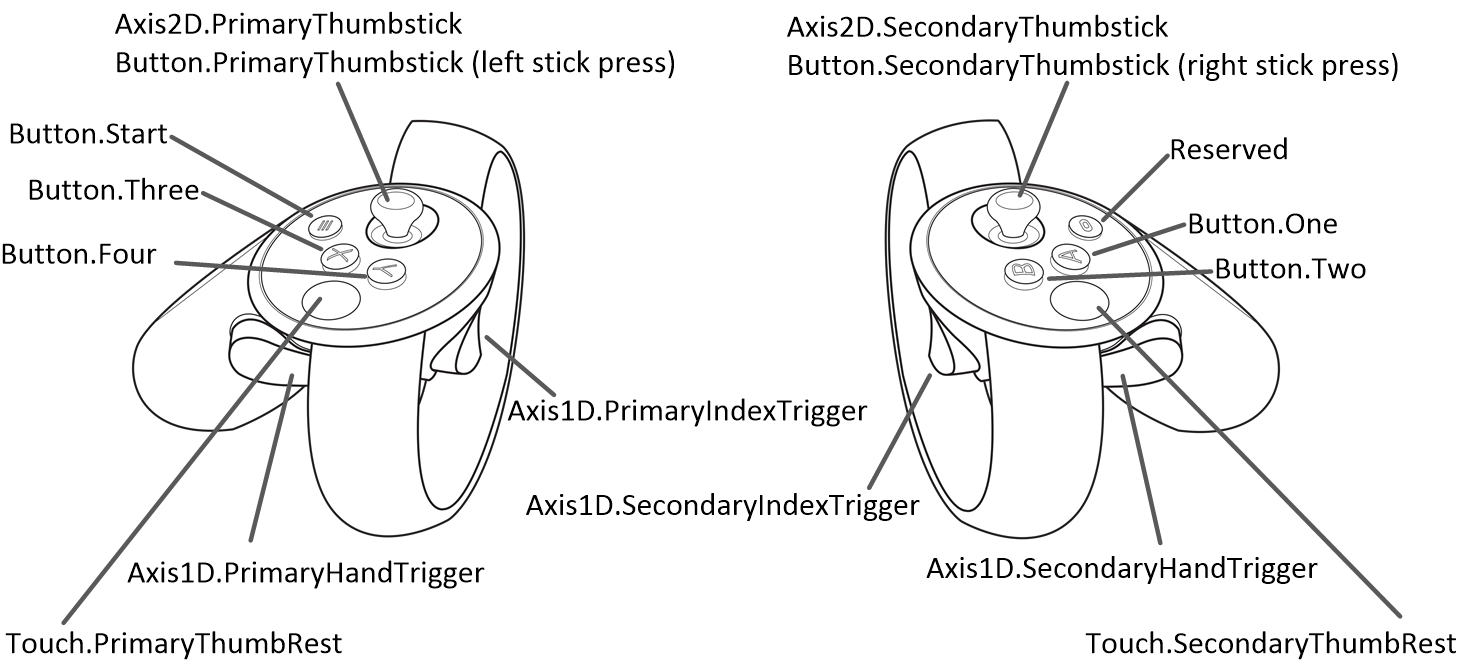
\includegraphics[width=13.5cm]{OculusTouch}
    \caption{Oculus Touch Controller mit der offiziellen Beschriftung von Oculus \cite{bib:OculusTouchPic}}
    \label{fig:OculusTouchPic}
\end{figure}

Der freie Flug-Modus ist die erste Navigationsart, die für C.LABEL-VR entwickelt wurde. Hierbei wurde vor allem auf den praktischen Nutzen für die Bewegung wert gelegt. Das Ziel war es also einen Bewegungsmodus zu implementieren, der für den Benutzer leicht verständlich und schnell zu erlernen ist. Außerdem sollte es möglich sein sich präzise zu Bewegen um leicht an gewünschte Positionen in der Punktwolke zu kommen.\\

Die Benutzereingabe für diesen Navigationsmodus erfolgt über die Analog-Sticks der Oculus Touch Controller (siehe \textit{Thumbstick} in Abbildung \ref{fig:OculusTouchPic}). Bewegt der Benutzer einen dieser Sticks, bewegt er sich auch in der virtuellen Welt. Wird der Stick wieder losgelassen, endet auch die Bewegung innerhalb der virtuellen Umgebung. Dies soll die gewünschte Intuitivität liefern. Die Längs- und die Lateral-Bewegung werden dabei mit dem linken Stick gesteuert. Durch Betätigung des rechten Sticks kann eine Vertikal-Bewegung oder eine Rotation um die eigene Achse ausgeführt werden. Die genauen Steueranweisungen sind in der Bedienungsanleitung zur Applikation zu finden (APPENDIX).\\

Um die Bewegungen aus dem Stand oder Richtungswechsel angenehmer für den VR-Benutzer zu machen wird im freien Flugmodus Beschleunigung und Verzögerung simuliert. Wird ein Steuerbefehl vom Benutzer gegeben, bewegt sich dieser nicht sofort mit voller Geschwindigkeit. Dies wäre ein, für den Menschen unnatürliches Bewegungsverhalten und könnte, zusätzlich zu den Auslösern aus Abschnitt \ref{sec:VRSickness}, zu Symptomen der VR-Krankheit führen. Stattdessen kommt die Bewegung, durch die Beschleunigung, langsam ins Rollen, sodass der Benutzer eine bestimmte Zeit hat um sich an die Geschwindigkeitsveränderung zu gewöhnen. Endet der Bewegungsbefehl, also lässt der Benutzer den entsprechenden Stick los, endet die Bewegung nicht schlagartig, sondern die Geschwindigkeit wird wie beim Bremsen mit einem Auto immer weniger, sodass auch hier der Benutzer Zeit hat sich an den Bewegungsstopp zu gewöhnen.      Besonders wichtig wird dieses Prinzip bei Richtungswechseln. Würde der Benutzer bei voller Geschwindigkeit einen Richtungswechsel vollziehen, bei dem er sich in die neue Richtung ebenfalls sofort mit Höchstgeschwindigkeit bewegt, würde dies in den meisten fällen zu Übelkeit führen, da der Richtungswechsel zu schlagartig vollzogen werden würde. Durch die Verzögerung kommt, bei einem Richtungswechsel, der Benutzer erst langsam zum Stehen und wird danach in die neue Richtung beschleunigt. Der Wechsel der Bewegungsrichtung wird also übergangsweise ausgeführt, was der VR-Krankheit entgegenwirkt. \\

Die Geschwindigkeit der Bewegung des Nutzers wird in jedem Update-Zyklus (erklärt in Abschnitt \ref{sec:UnityDevelopment}) der Applikation berechnet. Das heißt die Funktion \textit{ComputeSpeed} aus der Auflistung \ref{lst:FreeFly} wird in jedem dieser Zyklen aufgerufen. Die Beschleunigung wird nun so simuliert, dass ein bestimmter Beschleunigungswert auf den aktuellen Geschwindigkeitswert addiert wird, bis die Maximalgeschwindigkeit erreicht ist. Gibt es keinen Bewegungsbefehl mehr, wird vom aktuellen Geschwindigkeitswert solange ein Verzögerungswert abgezogen, bis die Geschwindigkeit null beträgt. Der Verzögerungswert ist in der Regel höher als der Beschleunigungswert, damit der Benutzer schneller zum Stehen kommt, als er Beschleunigt. Dies hat den Zweck dass der Anhaltevorgang präzise bleibt und der Benutzer so nicht zu weit verzögert bis er zum stehen kommt. Beide Werte können allerdings vom Benutzer selbst eingestellt werden (siehe Kapitel \ref{sec:AppMenu}). Der Richtungswechsel ist vom Prinzip her ähnlich implementiert. Hierbei wird allerdings ein noch höherer Subtrahend als der Verzögerungswert von der aktuellen Geschwindigkeit abgezogen, damit der Richtungswechsel schnell von statten geht, jedoch immer noch verzögert.

\begin{lstlisting}[caption={Vereinfachte Implementierung des Beschleunigungs- und Verzögerungsprinzip in eine einzelne Richtung}, captionpos=t, numbers=left, label=lst:FreeFly]
private float ComputeSpeed(bool move, float currentSpeed, float maxSpeed ,float accelerationValue, float decelerationValue)
{
	float newSpeed;	
	
	if(move == true)
	{
		if(currentSpeed < maxSpeed)
			newSpeed = currentSpeed + accelerationValue;
		else
			newSpeed = maxSpeed;
	}
	else
	{
		if(currentSpeed > 0)
			newSpeed = currentSpeed - decelerationValue;
		else
			newSpeed = 0;
	}
	
	return newSpeed;
}
\end{lstlisting}
\quad

Durch den freien Flugmodus soll dem Benutzer eine Bewegungsart zur Verfügung gestellt werden, die den gewohnten Bewegungsabläufen des Menschen ähnelt. Dies ist mit der Simulation von Beschleunigung und Verzögerung gegeben. Durch einen höheren Verzögerungswert kann darüber hinaus sichergestellt werden, dass der Benutzer präzise an eine gewünschte Position navigieren kann. Nichts desto trotz kann es bei diesem Bewegungsmodus dazu kommen, dass Symptome der VR-Krankheit auftreten. Dies kommt daher, dass der Mensch eine konstante Bewegung visuell wahrnimmt, sie aber nicht körperlich fühlt (vgl. Abschnitt \ref{sec:VRSickness}). Um diesen Nachteil auszugleichen wurde zusätzlich noch ein zweiter Navigationsmodus entwickelt.
 
\subsection{Teleport-Modus}
\label{sec:TeleportMode}

Der Teleport-Modus ist der zweite Navigationsmodus der für C.LABEL-VR entwickelt wurde. Der Zweck dieses Modus ist es, die Anfälligkeit des freien Flug-Modus (Abschnitt \ref{sec:FreeFlyMode}) für die VR-Krankheit auszugleichen. Symptome der VR-Krankheit treten beim freien Flug auf, da der Benutzer eine konstante Bewegung auf visuellem Weg wahrnimmt, jedoch nicht mit dem Gleichgewichtssinn spürt. Durch Teleportation, also den unverzögerten Sprung von einer Position zu einer anderen, gibt es keine konstante Bewegung. So soll nun der VR-Krankheit entgegen gewirkt werden. Diese Art der Bewegung ist aktuell die am weitesten verbreitet unter VR-Anwendungen \cite{bib:VRLocomotionReview}, da sie nachweislich weniger anfällig für die VR-Krankheit ist \cite{bib:PointTeleport}.\\

Das Prinzip der Steuerung ist ähnlich wie das des freien Flug-Modus. Steuerungsbefehle kann der Benutzer zunächst mit den Sticks tätigen (siehe \textit{Thumbstick} in Abbildung \ref{fig:OculusTouchPic}). Auch hier wird die Längs- und die Lateral-Bewegung mit dem linken und die Vertikal- und Rotations-Bewegung mit dem Rechten Stick gesteuert. 

TODO TEXT abklären
-------Die genauen Steueranweisungen sind in der Bedienungsanleitung zur Applikation zu finden (APPENDIX).-----------\\

Wie schon erwähnt gibt es, im Gegensatz zum freien Flug-Modus, keine konstante Bewegung durch die Benutzereingaben. Stattdessen wird die Position des Benutzers in der virtuellen Welt durch die Steuerbefehle unverzögert verschoben, sodass es einem Teleport gleicht. Die Implementation dieses Vorgangs ist dank der Transform-Komponente eines Gameobjects (siehe Abschnitt \ref{sec:UnityDevelopment}) nicht aufwändig. Wie in der Auflistung \ref{lst:Teleport} zu sehen ist, kann die Verschiebung des Objekts \textit{userView} um einen Vektor mit einem einzigen Befehl vollzogen werden. Dieses Objekt repräsentiert dabei die Augen des Benutzers in der virtuellen Welt. Wird es also verschoben, ist es für den Benutzer so, als würde er von einer zur anderen Position teleportiert werden. Der Vektor um den der Benutzer verschoben wird, kann von ihm selber eingestellt werden (siehe Kapitel \ref{sec:AppMenu}).

\begin{lstlisting}[caption={Implementierung des Teleportationsbefehls}, captionpos=t, numbers=left, label=lst:Teleport]
GameObject userView;

userView.transform.Translate(new Vector3(xDirection, yDirection, zDirection));
\end{lstlisting}
\quad

\begin{figure}%
    \centering
    \subfloat[Vor dem Teleport]{\fbox{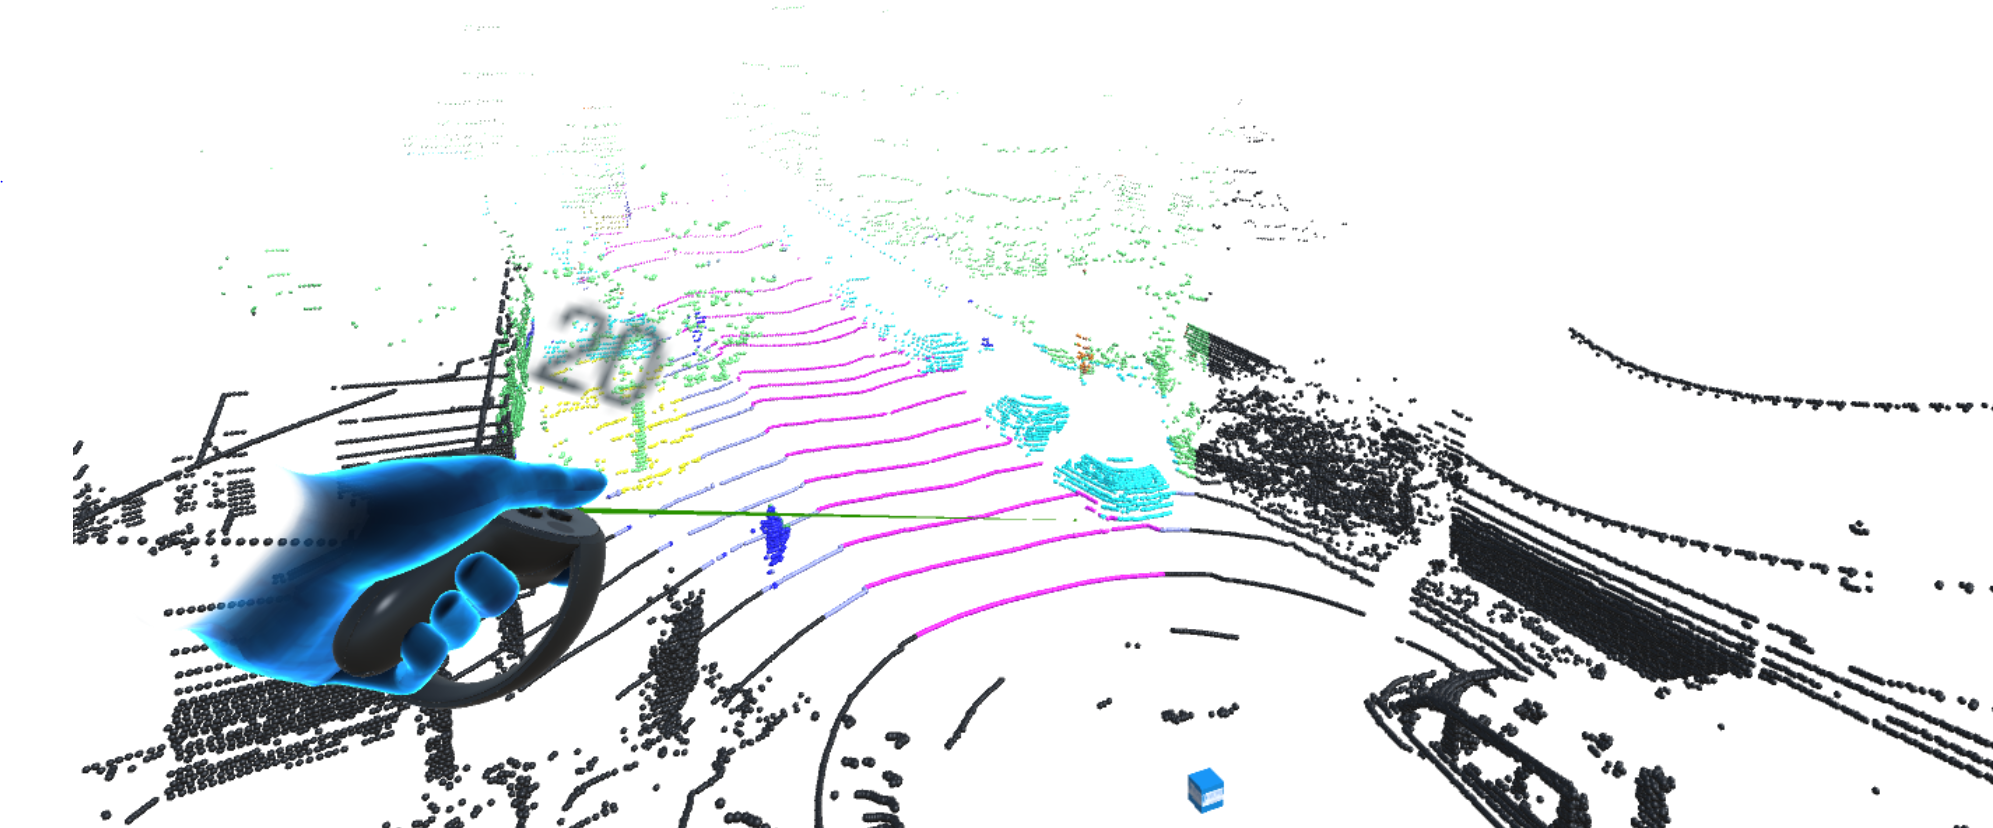
\includegraphics[width=12cm]{PointerTeleportPre}\label{fig:PointerTeleportPre}}}%
    \qquad
    \subfloat[Nach dem Teleport]{\fbox{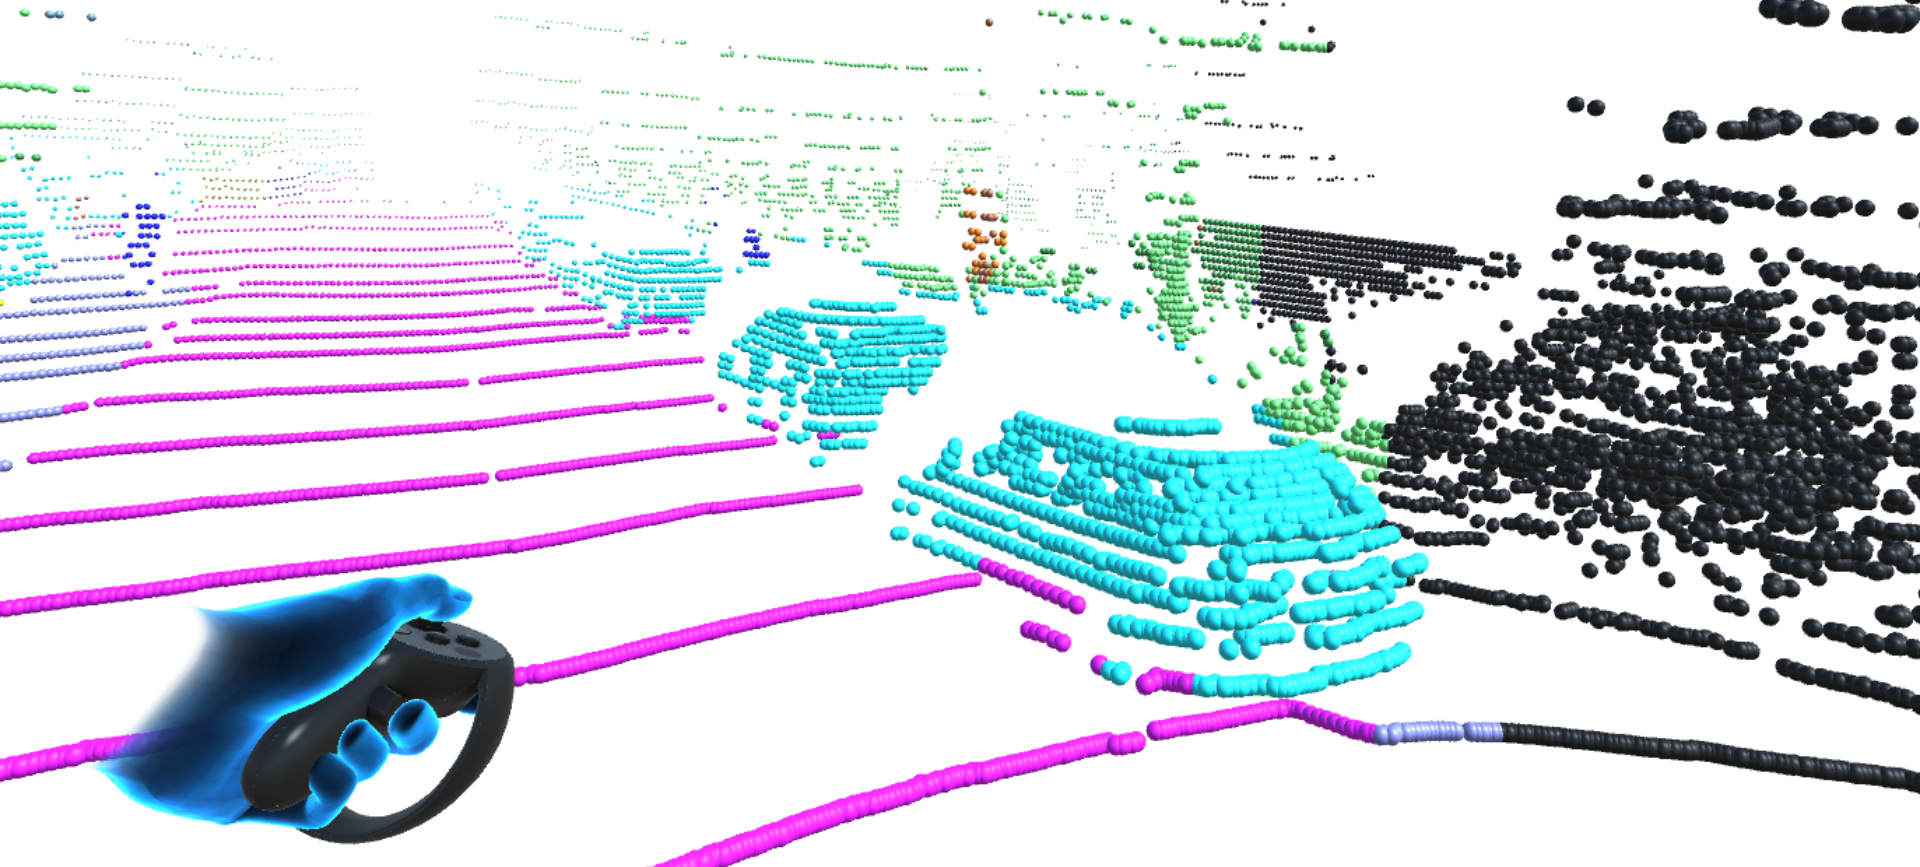
\includegraphics[width=12cm]{PointerTeleportAfter}\label{fig:PointerTeleportAfter}}}%
    \caption{Zu sehen ist der Vorgang eines Pointer-Teleports.}
    \label{fig:Components}%
\end{figure}

Zusätzlich zu den Benutzereingaben durch den Stick, gibt es eine weitere Möglichkeit für den Benutzer sich an eine bestimmte Stelle in der virtuellen Welt zu teleportieren. Dazu kann er eine Art Laserstrahl aktivieren, der vom linken virtuellen Controller ausgeht (Abbildung \ref{fig:PointerTeleportPre}). Dieser Strahl fungiert wie eine Stange die der Benutzer in der Hand hält, sie bewegt sich also mit der Handbewegung des Nutzers mit. Der Strahl kann durch die Hand-Auslöser-Taste des linken Controllers aktiviert werden (siehe \textit{PrimaryHandTrigger} in Abbildung \ref{fig:OculusTouchPic}). Dabei wird auch die Länge des Strahls angezeigt, was ebenfalls in der Abbildung \ref{fig:PointerTeleportPre} zu sehen ist. Die Länge des Strahls kann anschließend vom Benutzer angepasst werden, indem er den linken Stick nach vorne (Strahl wird länger) oder nach hinten (Strahl wird kürzer) drückt. Betätigt der Benutzer die Index-Auslöser-Taste (\textit{PrimaryIndexTrigger} in Abbildung \ref{fig:OculusTouchPic}) wird er an die Spitze des Laserstrahls teleportiert (vgl. Abbildung \ref{fig:PointerTeleportAfter}). Mit Hilfe dieser Teleportationsart kann der Benutzer auch große Distanzen in der virtuellen Welt, schnell zurücklegen. Für die Implementation dieser Funktion kann ebenfalls der Befehl aus der Auflistung \ref{lst:Teleport} verwendet werden, wobei statt dem neu erzeugten Vektor die Position des Strahlendes verwendet wird.\\

Durch die Bewegung mittels Teleport wird also der VR-Krankheit entgegengewirkt, da es keine konstante Bewegung für den Benutzer gibt. Durch den Teleport mittels Laserstrahl können hierbei auch große Distanzen vom Benutzer zurückgelegt werden. Der Nachteil dieses Bewegungsmodus ist es, dass durch feste Teleportationsdistanzen keine präzise Stuerung mehr garantiert werden kann. Da aber genau dafür der freie Flug-Modus Abhilfe schafft, ergänzen sich die beiden Navigationsmodi sehr gut und bieten dem Benutzer so passende Möglichkeiten sich durch die virtuelle Welt zu Bewegen.
 

\section{Annotieren der Punktwolke}
\label{sec:Annotation}
Nachdem im vorherigen Kapitel Möglichkeiten erläutert wurden, wie man durch eine VR-Punktwolke navigieren kann, gilt es nun Punkte aus dieser Wolke zu annotieren. Dazu wurden drei verschieden Möglichkeiten implementiert. Alle drei basieren zunächst auf Kollisionserkennungen, bei denen erkannt wird, dass ein Objekt mit einem Punkt der Wolke kollidiert. Auf diese Weise können Punkte mit einem anderen Objekt ausgewählt werden um diese anschließend zu annotieren. Die Auswahl erfolgt, beispielsweise bei der Pointer Annotation in Kapitel \ref{sec:SimplePointerAnnotation}, mit einer Art Laserpointer. Die Interaktion mit Objekten innerhalb von VR-Applikationen erfolgt oft über derartige Pointer \cite{bib:OftenPointerUse}. Eine andere Art der Auswahl ist die Berührung eines Punktes mit dem virtuellen Controller. Da sich der virtuelle Controller wie der physische Controller verhält, den der Benutzer in der Hand hält, ist es so, als würde der Benutzer den Punkt selbst berühren. Dieses Verfahren nennt sich \textit{Touch Annotation} und wird in Kapitel \ref{sec:TouchAnnotation} beschrieben. Die dritte Art der Annotation bietet die Möglichkeit, einen ganzen Cluster von Punkten auf einmal zu annotieren. Dazu annotiert der Benutzer einen einzelnen Punkt mit einem Pointer. Ist während dessen die CLuster-Annotation aktiviert, wird dieser Punkt als Startpunkt benutzt und ein Algorithmus sucht sich alle umliegenden Punkte, die zum gleichen Objekt gehören wie der Startpunkt. Alle gefundenen Punkte werden auf einmal annotiert. Die Funktionsweise dieses Algorithmus wird im Kapitel \ref{sec:GroundPointSegmentation} erläutert.\\

Um die Punkte mit einer bestimmten Klassifikation zu versehen, muss erst die richtige Klasse ausgewählt werden. Der Name der aktuell ausgewählten Klasse wird stets über dem rechten Controller angezeigt (vgl. Abbildung \ref{fig:PointerAnnotation}). Zur Auswahl der gewünschten Klassifikation gibt es in C.LABEL-VR zwei Möglichkeiten. Zum einen kann der Benutzer mit den Tasten \textit{One} und \textit{Two} aus Abbildung \ref{fig:OculusTouchPic} durch die vorhandenen Klassen iterieren. Eine andere Möglichkeit ist die Nutzung einer Funktionsweise die einer Pipette ähnelt. Dazu wird mit dem Pointer ein Punkt mit der gewünschten Label anvisiert und anschließen die Pipetten-Funktion mit dem Drücken des \textit{SecondaryThumbstick} aktiviert. Die aktuell ausgewählte Klassifikation wird somit durch die Klassifikation des anvisierten Punktes ersetzt. Auf diese zwei Arten kann der Benutzer das gewünschte Label auswählen, um anschließend Punkte mit diesem zu annotieren.

\subsection{Pointer Annotation}
\label{sec:SimplePointerAnnotation}
Die erste Annotationsmöglichkeit, die für C.LABEL implementiert wurde, ist die Pointer Annotation. Der Name dieser Annotationsart kommt daher, dass damit Punkte mit einer Art Laserpointer annotiert werden können. Solch ein Pointer ist auch schon beim Pointer Teleport im vorherigen Abschnitt \ref{sec:TeleportMode} vorgestellt worden. Der Pointer besteht dabei aus einem Strahl und einer Kugel (\textit{Cursor}) am Ende des Strahls. Er geht vom rechten Controller aus und wird mit dem \textit{SecondaryHandTrigger} aktiviert (siehe Abbildung \ref{fig:OculusTouchPic}). Wird diese Taste wieder losgelassen, wird der Pointer deaktiviert und ist somit nicht mehr sichtbar. Mit Hilfe des aktivierten Pointers, kann der Benutzer einen Punkt anvisieren, den er annotieren möchte. Ist der gewünschte Punkt anvisiert, so wird er, durch Betätigung des \textit{SecondaryIndexTrigger}, mit der aktuell ausgewählten Klassifikation versehen. Die Abbildung \ref{fig:PointerAnnotation} zeigt diesen Prozess.\\ 

\begin{figure}%
	\centering
    \fbox{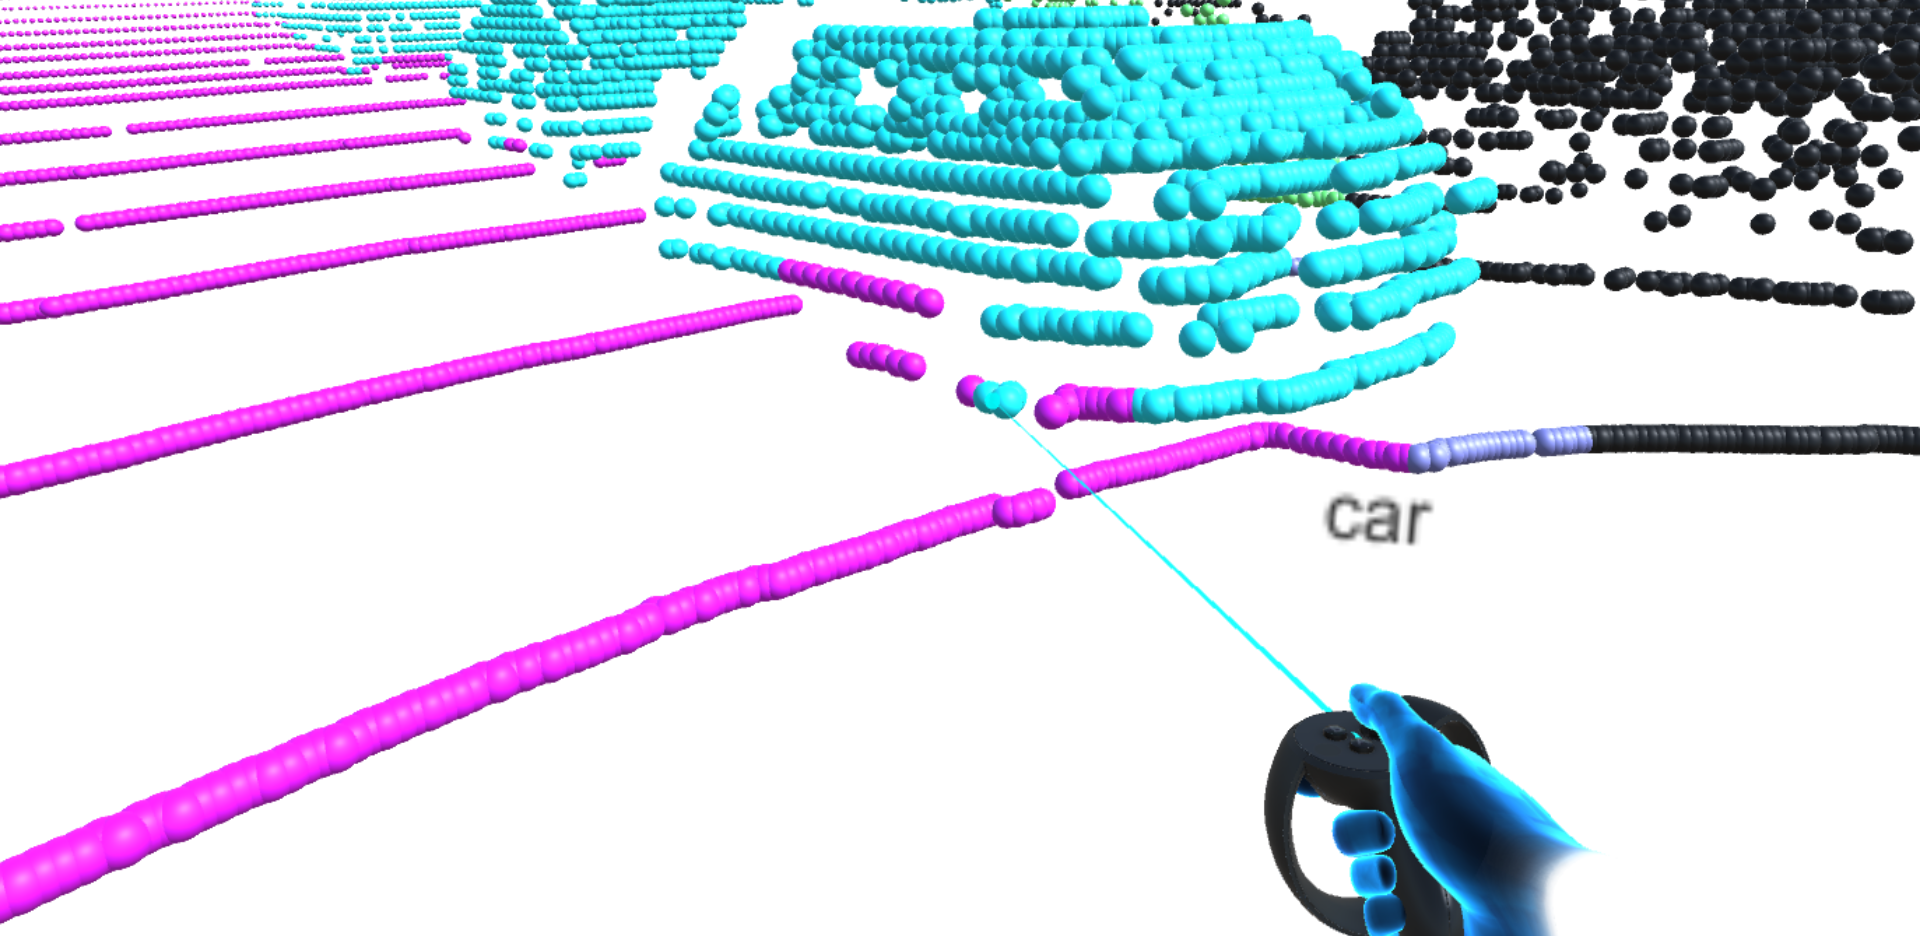
\includegraphics[width=15cm]{PointerAnnotation}}
    \caption{Annotation eines Punktes mit der Klasse \textit{Car}, durch eine Pointer-Annotation}
    \label{fig:PointerAnnotation}
\end{figure}

Um das Annotieren mit solch einem Pointer zu realisieren, sind zwei Hauptfunktionen zu implementieren. Zum einen ist dies die dynamische Anpassung der Pointer-Länge beim Auftreffen des Pointers auf Objekte und zum anderen die Identifikation der Objekte, mit dem der Pointer kollidiert, wenn ein Annotationsbefehl gegeben wird. Die Anpassung der Pointer-Länge geschieht über ein \textit{Raycasting}. Ein Ray ist in Unity eine Halbgerade, die von einem Ursprung in eine bestimmte Richtung verläuft. Im falle des Pointers wird ein Ray initialisiert, der seinen Ursprung vorne am Controller hat (über dem IndexTrigger) und längs aus dem Controller heraus verläuft. Ursprung und Richtung des Rays passen sich immer der Position und Orientierung des Controllers an, sodass dieser immer längs aus dem Controller heraus verläuft. Entlang dieses Rays kann der Pointer gezeichnet werden. Ursprung und Orientierung des Pointers ist also die gleiche, wie die des Rays.\\ 

Die Physik-Engine von Unity bietet eine Funktion zur Überprüfung, ob solch ein Ray mit einem Objekt kollidiert, das eine Collider-Komponente hat \cite{bib:UnityRaycast}. Dies ist eine von mehreren Arten der Kollisionserkennung in Unity. In Kapitel \ref{sec:Generierung} wurde schon erwähnt, dass jeder Punkt einer Punktwolke in C.LABEL-VR eine solche Collider-Komponente besitzt. Somit kann überprüft werden, ob der Pointer mit einem Punkt der Wolke kollidiert. Ist dies der Fall gibt die Überprüfungsfunktion der Physik-Engine die Information zurück um welchen Punkt es sich handelt und an welcher genauen Position (\textit{x, y, z}) der Treffer des Rays anliegt. Durch diese Information kann die Länge des Poniters angepasst werden. Orientierung und Verlauf des Pointers bleiben gleich, jedoch entspricht der Pointer nicht mehr einer Halbgeraden, sondern einer Strecke vom Controller zum Ort der Kollision am Punkt. Der Cursor des Pointers befindet sich somit am Kollisionsort zwischen Pointer und dem Punkt.\\

Zeigt der Pointer des Controllers auf diese Weise auf einen Punkt, so ist dieser Punkt vom Benutzer anvisiert. Nun kann der Benutzer mit dem \textit{SecondaryIndexTrigger} einen Annotationsbefehl geben. Tut er dies, wird die Kollisionserkennung zwischen dem Cursor des Pointers und allen anderen Objekte aktiviert. Diese Kollisionserkennung ist auf Basis zweier Objekte und nicht, wie bei der Längenanpassung, zwischen einem Ray und einem Objekt\cite{bib:UnityPhysics}. Mit dieser Art der Kollisionserkennung ist es möglich, unter bestimmten Voraussetzungen, Kollisionen zwischen zwei Objekten zu erkennen. Dabei werden bestimmte Aktionen ausgelöst, wie das Senden einer Kollisionsnachricht oder die Positionsänderung der kollidierten Objekte, auf Basis der Kollisionseigenschaften der Objekte. Da die Punkte in einer Punktwolke bei einer Kollision nicht bewegt werden sollen, ist ihnen eine statische Collider-Komponente zugeordnet (siehe Kapitel \ref{sec:Generierung}). Diese Komponente besagt, dass das Objekt bei einer Kollision nicht bewegt werden muss \cite{bib:Collider}. Somit müssen auch keine physikalischen Berechnungen durchgeführt werden, was Rechenzeit spart.\\

Eine Voraussetzung für diese Art Kollisionserkennung ist beispielsweise das Vorhandensein einer Collider-Komponente beim einen Objekt und einer Rigidbody-Komponente beim anderen. In \cite{bib:Collider} sind alle anderen Voraussetzungen genannt, unter denen Kollisionen erkannt werden können. Eine Rigidbody-Komponente kontrolliert die Positionsänderung eines Objekts bei einer Kollision mit einem anderen, wenn das andere Objekt die passende Collider-Komponente hat \cite{bib:UnityRigidBody}. Da die Punkte der Wolke eine statische Collider-Komponente haben, ist dem Cursor des Pointers, der auch ein Objekt ist, die passende Rigidbody-Komponente zugeordnet. Gibt nun der Benutzer den Annotationsbefehl, wird durch die Rigidbody-Komponente überprüft, mit welchen Collider-Komponenten der Cursor kollidiert.\\

Anhand dieser Komponenten kann festgestellt werden, welchen Objekten diese zugeordnet sind. So kann überprüft werden, bei welchen dieser Objekte es sich um einen Punkt der Punktwolke handelt. Ist dies der Fall kann von jedem Punkt auf die jeweilige IDS-Komponente (siehe Kapitel \ref{sec:Generierung}) zugegriffen werden, in der die Information über das Label des Punktes zu finden ist. Das Label kann auf diese Weise durch das aktuell ausgewählte Label ersetzt werden. Somit werden alle Punkte annotiert die, beim Annotationsbefehl des Benutzers, mit Hilfe des Pointers anvisiert sind.

\subsection{Touch Annotation}
\label{sec:TouchAnnotation}

\begin{figure}%
	\centering
    \fbox{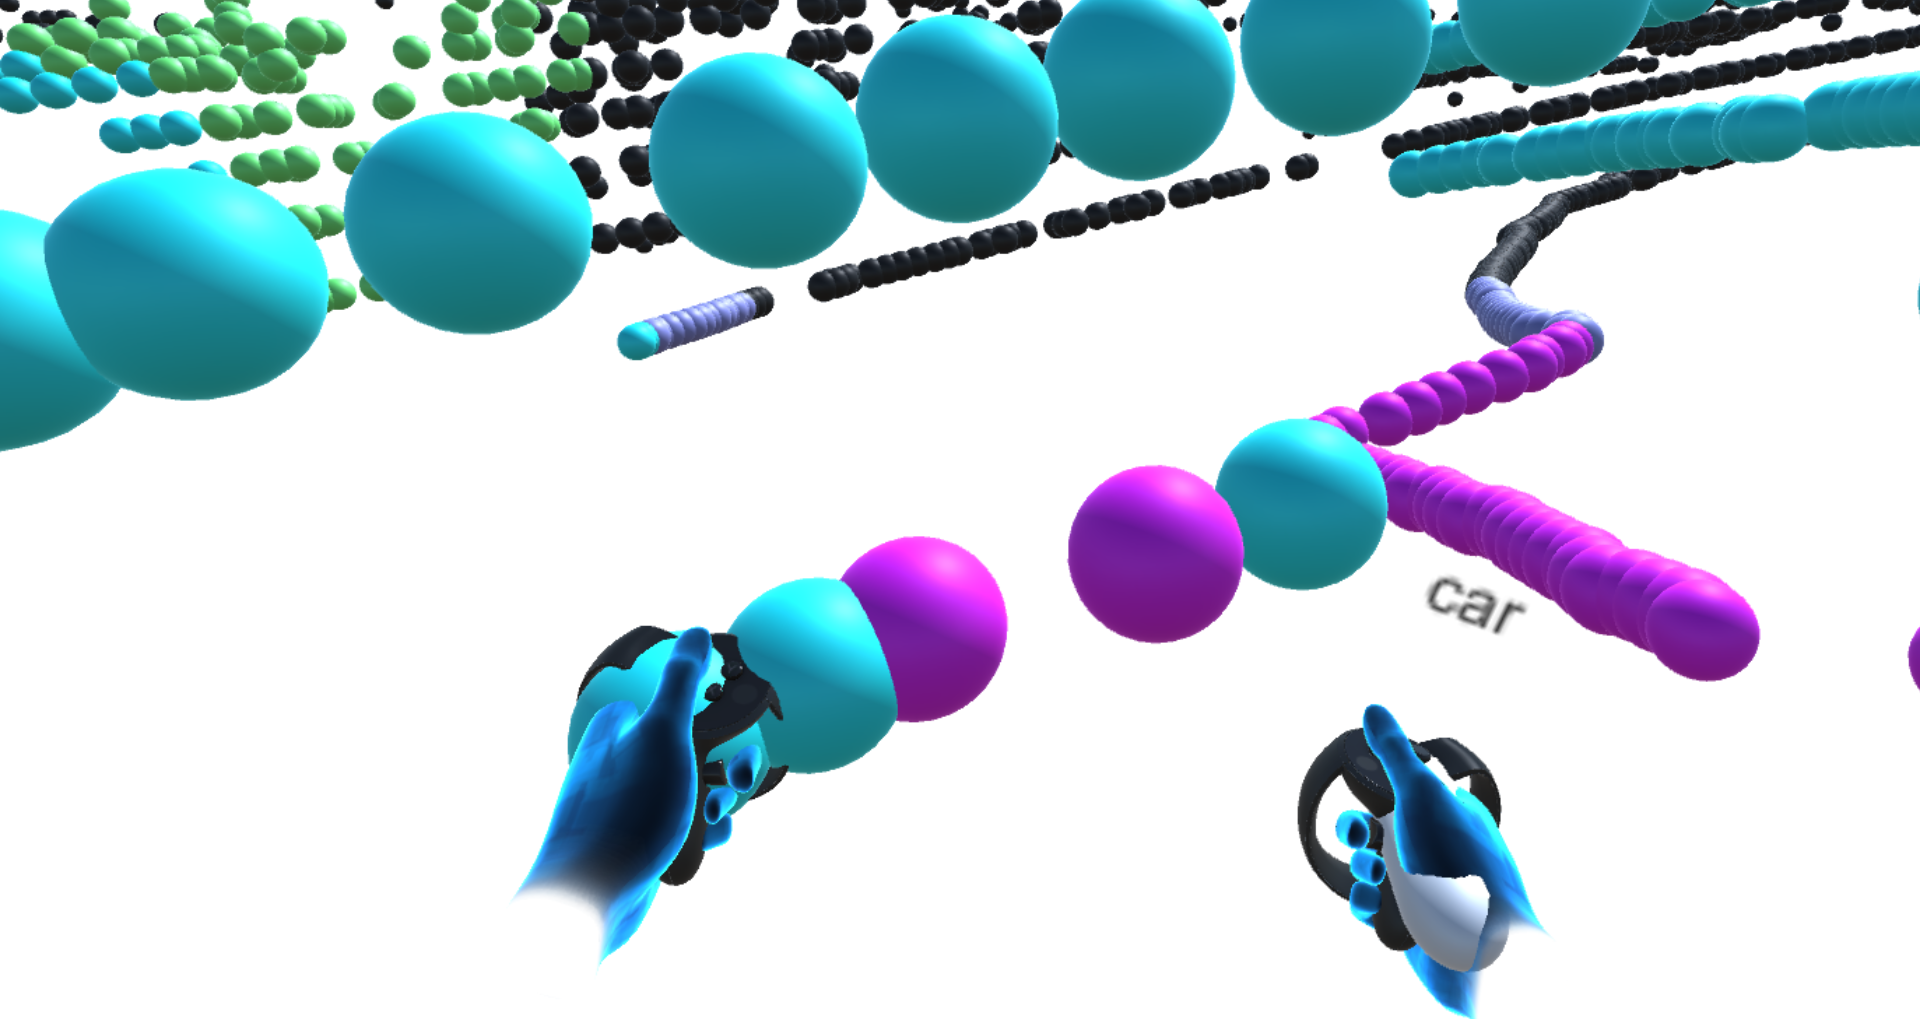
\includegraphics[width=15cm]{TouchLabeling}}
    \caption{Abbildung eines Touch Annotations-Vorgang. Mit der linken Hand wird eine Punkt berührt, der dadurch klassifiziert wird.}
    \label{fig:TouchLabeling}
\end{figure}

In Kapitel \ref{sec:WhyVR} wurde schon angemerkt, dass die Applikation auch für Marketingzwecke dienen soll, beispielsweise auf Messen, um Kunden auf das Unternehmen CMORE und dessen Prdoukte und Dienstleistungen aufmerksam zu machen. Dafür bietet sich die Virtual Reality Technologie an, da sie größtenteils immer noch als neuartig und deswegen als interessant angesehen wird. Damit C-LABEL-VR die Virtual Reality Technologie ausnutzt, wurde ein Annotationsmodus implementiert, der in dieser Form nur mit einem VR-System möglich ist. Gemeint ist damit die \textit{Touch Annotation}. Mit ihr ist es möglich, durch Berührung der Punkte mit dem virtuellen Controller, diese zu annotieren. Bewegt der Benutzer also seine Hand in Richtung eines Punktes, bewegt sich der virtuelle Controller ebenfalls in diese und sobald dieser den Punkt berührt, wird er annotiert (siehe Abbildung \ref{fig:TouchLabeling}). In diesem Moment wird dem Benutzer per Controller-Vibration eine haptische Rückmeldung gegeben. Dies führt für den Benutzer zu der Immersion, dass er den Punkt berühren würde.\\

Das Funktionsprinzip dahinter ist, ähnlich wie bei der Pointer Annotation in Abschnitt \ref{sec:SimplePointerAnnotation}, eine Kollisionserkennung. Kollidiert der Controller mit einem Punkt der Punktwolke, wird dieser mit dem aktuell ausgewählten Label annotiert. Die virtuellen Controller, Hände und deren Funktionen werden vom \textit{Oculus Avatar SDK} zur Verfügung gestellt \cite{bib:AvatarSDK}. Diese beinhalten keine Kollisionsmechanismen, da diese spezifisch für jede Entwicklungsplattform erstellt werden müssen. Um dies zu bewerkstelligen wird jedem Controller ein Kind-Objekt (siehe Kapitel \ref{sec:UnityDevelopment}) in Form eines 3D-GameObjects (genannt \textit{Toucher}) angehängt, welches sich an der gleichen Position wie der Controller befindet. In der Abbildung \ref{fig:TouchLabeling} ist ein solches Objekt am rechten Controller zu sehen (weißes Objekt im rechten Controller). Das Objekt wurde aber nur zu Anschauungszwecken eingeblendet. Im normalen Betrieb ist dieses Objekt nicht zu sehen. Durch die Eltern-Kind-Beziehung bewegt sich dieses Objekt stets mit dem Controller mit.\\

Das Objekt wird zusätzlich mit einer Rigidbody-Komponente ausgestattet. Dadurch kann eine Kollision mit einem anderen Objekt, welches eine Collider-Komponente besitzt, von der Physik-Engine von Unity festgestellt werden. Dies ist das selbe Prinzip, das auch bei der Pointer Annotation aus Kapitel \ref{sec:SimplePointerAnnotation} benutzt wurde. Bewegt der Benutzer also den virtuellen Controller solange zu einem Punkt in der Punktwolke, bis dieser ihn erreicht, berührt der angehängte Toucher diesen Punkt. In diesem Fall wird eine Kollision zwischen Toucher und Punkt festgestellt.\\

Bei einer Kollision des Touchers mit anderen Objekten wird jedes Kollisionsobjekt überprüft, ob es sich um einen Punkt der Punktwolke handelt. Ist dies der Fall wird, wie im vorherigen Abschnitt \ref{sec:SimplePointerAnnotation}, auf die IDS-Komponente des Punktes zugegriffen und das Label in der Komponente, mit dem aktuell ausgewählten ersetzt. Um den Toucher, der sich an der gleichen Position wie der virtuelle Controller befindet, nicht als störend zu empfinden, wird die Mesh Renderer-Komponente dieses Objekts deaktiviert. Somit wird die Visualisierung des Objektes ausgeschaltet, wobei die restlichen Funktionen des Objekts und dessen Komponenten aktiv bleiben. Somit sieht es für den Benutzer aus, als würde die Kollisionserkennung vom Controller aus gehen. 


\subsection{Cluster Annotation}
\label{sec:ClusterLabeling}
In einer Punktwolke mit mehreren tausend Punkten wird es für den Benutzer auf Dauer mühsam jeden Punkt einzeln zu Annotieren. Bei diesem Problem soll die \textit{Cluster Annotation} Abhilfe schaffen. Diese Art der Annotation soll selbstständig diejenigen Punkte in einen Cluster aufnehmen und sie mit der gleichen Klasse labeln, die zum gleichen Objekt gehören. Der Benutzer wählt hierfür, wie im vorherigen Kapitel \ref{sec:SimplePointerAnnotation} einen Punkt mit Hilfe des Pointers aus. Ausgehend davon werden umliegende Punkte untersucht, ob sie zum gleichen Objekt gehören wie der ausgewählte Startpunkt. Ist dies der Fall werden sie in den Cluster aufgenommen. Werden keine Punkte mehr aufgenommen bleibt der Endcluster übrig, welcher dann einem Objekt entspricht, zum Beispiel einem Auto. \\

Wissenschaftler beschäftigen sich intensiv mit solchen Verfahren zur Objektidentifizierung in dreidimensionalen Punktwolken. Ansätze, wie sie in \cite{bib:Segmentation1}, \cite{bib:Segmentation2} oder \cite{bib:Segmentation3} vorgestellt werden sind nur wenige von vielen. Die meisten haben aber ein ähnliches Vorgehen. Zuerst werden all diejenigen Punkte in der Wolke entfernt, die zum Boden gehören. So bleiben anschließend nur noch Punkte übrig, welche zu Objekten wie beispielsweise Autos, Häuser oder Straßenschilder gehören. Die übrigen Punkte können nun mit diversen Algorithmen zu Clustern zusammengefasst werden. Ein Beispiel für das Ergebnis eines solchen Verfahrens bietet die Abbildung \ref{fig:ClusteredCloud}. Im Folgenden wird vorgestellt wie die Cluster-Analyse in C.LABEL-VR funktioniert.

\begin{figure}%
	\centering
    \includegraphics[width=15cm,height=7cm]{ClusteredPointCloud}
    \caption{Objektidentifizierung einer 3D-Punktwolke aus \cite{bib:Segmentation1}. Die Bodenpunkte der Wolke sind blau dargestellt und die Objekte sind mit Boxen gekennzeichnet.}
    \label{fig:ClusteredCloud}
\end{figure}

\subsubsection{Bodenpunkt-Analyse}
\label{sec:GroundPointSegmentation}
Wie schon erwähnt werden bei vielen Verfahren der Cluster-Analyse von Punktwolken zuerst die Bodenpunkte identifiziert. Dieses Verfahren wird auch in dieser Arbeit angewendet. Der Grund dafür ist, dass die Bodenpunkte nicht in das Suchverfahren nach Objektpunkten aufgenommen werden dürfen. Sie würden nicht nur die Suche nach echten Objektpunkten erschweren sondern auch das Ergebnis der Objektcluster verfälschen. Als Erklärung soll folgender, simpler Cluster-Algorithmus dienen:

\begin{enumerate}
\item Definiere einen Startpunkt $p$.
\item Ausgehend von $p$, suche alle Punkte innerhalb von Radius \(x\). 
\item Jeder gefundene Punkt ist ein neuer Startpunkt $p$.
\item Führe 2. aus bis es keine neuen Punkte $p$ mehr gibt.
\end{enumerate} 

Alle Objekte die auf dem Boden stehen, also deren Punkte nahe an Bodenpunkten sind, würden mit dem obigen Algorithmus die Bodenpunkte mit in den Cluster aufnehmen. Dies kann sogar dazu führen, dass 2 Objekte, die mittels Bodenpunkten miteinander verbunden sind zu einem Cluster zusammengefügt werden. Darum müssen die Bodenpunkte von den Objektpunkten getrennt werden um eine exakte Objekterkennung zu garantieren.

Die Segmentierung des Bodens wird in C.LABEL-VR nach dem Einlesen des internen Datenformates ausgeführt, also zwischen Import Addons und PCL Generator (siehe Abbildung \ref{fig:ImportExport}). Beim Erstellen der Punktwolken ist also schon bekannt welcher Punkt ein Bodenpunkt ist und welcher nicht. Dazu wird im internen Datenformat das Attribut für die Bodenpunktkennzeichnung mit dem entsprechenden Wert versehen (vgl. Abschnitt \ref{sec:IDS}). Wie diese Werte ermittelt werden ist im Folgenden erklärt.\\

Als Basis für die Bodenpunktanalyse in C.LABEL-VR wurde das \textit{Ground Plane Fitting}-Verfahren (GPF) aus \cite{bib:Segmentation1} verwendet. Ist im weiteren Verlauf dieser Arbeit die Rede von GPF, ist immer der Ansatz der eben zitierten Arbeit gemeint. Ziel dieses Verfahrens ist es ein mathematisches Modell einer Ebene zu errechnen, welches den Boden repräsentieren soll. Anschließend kann von jedem Punkt der Abstand zu dieser Ebene ermittelt werden. Ist der Abstand eines Punktes kleiner als ein definierter Wert, so handelt es sich bei ihm um einen Bodenpunkt.

Die Punktwolke, die analysiert werden soll, wird dabei zunächst in eine Anzahl an $N_{segs}$ Segmenten aufgeteilt. Der Algorithmus zur Identifizierung der Bodenpunkte wird für jedes dieser Segmente ausgeführt. Der Grund für diese Segmentierung ist die mögliche Unebenheit der Bodenfläche. Soll eine wellige Oberfläche von einer Ebene repräsentiert werden kommt es zu ungenauen Ergebnissen. Wird aber für jedes Segment der Punktwolke eine eigene Ebene ermittelt so verbessert sich das Ergebnis der Bodenpunktanalyse, wie in Abbildung \ref{fig:Segments} zu sehen ist.

\begin{figure}%
	\centering
    \includegraphics[width=14cm,height=6cm]{Segments}
    \caption{In \cite{bib:Segmentation1} wird gezeigt, dass die Segmentierung einer Punktwolke zu einem besseren Ergebnis der Bodenpunktanalyse führt. Die obere Abbildung ist dabei ohne Segmentierung und die untere mit Segmentierung. Bodenpunkte sind blau und Objektpunkte in grün dargestellt. Die roten Rechtecke kennzeichnen den Bereich in dem die Analyse schlechter bzw. besser ist.}
    \label{fig:Segments}
\end{figure}

Beim GPF-Verfahren wurden Punktwolken in 3 große Segmente entlang der $x$-Achse eingeteilt, da diese Achse der Fahrtrichtung des Autos entspricht. Damit wurden für die Testdaten, die CMORE für diese Arbeit zur Verfügung stellte, keine zufriedenstellenden Ergebnisse erzielt (vgl. Abbildung \ref{fig:WrongSegments}). Das Problem ist, dass sich durch eine zu simple Segmentierung entweder zu viele oder zu wenige Bodenpunkte in einem Sektor befinden können. Bei zu vielen Bodenpunkten kann es sein, dass der Boden nicht linear verläuft. Auf der linken Seite des Autos könnte sich beispielsweise eine Anhöhe befinden und auf der rechten Seite ein flaches Gelände. In diese Unebenheit kann keine richtige Ebene eingesetzt werden. Bei zu wenigen Bodenpunkten kann es sein, dass der Algorithmus die Ebene an Objekte annähert. Handelt es sich bei solchen Objekten beispielsweise um eine senkrechte Wand, können die vielen hohen Punkte die Ebene senkrecht werden lassen(siehe Abbildung \ref{fig:WrongFit}).\\

\begin{figure}%
    \centering
    \subfloat[Segmentierung anhand potentieller Bodenpunkten]{{\includegraphics[width=7cm]{GroundSeg_BirdeyeWithSectors2}\label{fig:RightSegments}}}%
    \qquad
    \subfloat[Segmentierung anhand Koordinaten entlang der $x$-Achse]{{\includegraphics[width=7cm]{GroundSeg_BirdeyeWithWrongSectors2}\label{fig:WrongSegments}}}%
    \caption{Vergleich der Segmentierungsmethoden zur Bodenpunktanalyse aus \cite{bib:Segmentation1} und C.LABEL-VR. Bodenpunkte sind rot, alle anderen schwarz. Die blauen Linien stellen die Trennung der Segmente dar. Die grünen Boxen markieren den Bereich, in dem man den Unterschied der beiden Methoden bei der Bodenpunkterkennung sieht.}\label{fig:Segmentation}%
\end{figure}

\begin{figure}%
	\centering
    \includegraphics[width=15cm,height=5cm]{WrongFit}
    \caption{Bei zu wenigen Bodenpunkten in einem Segment passt sich die Ebene den falschen Punkten an.}
    \label{fig:WrongFit}
\end{figure}

Darum wurde in dieser Arbeit ein Verfahren entwickelt, dass die Segmente nicht anhand ihrer Größe einteilt sondern nach der Anzahl der potentiellen Bodenpunkte, welche die Segmente enthalten (siehe Algorithmus \ref{alg:Segmentation}). Potentielle Bodenpunkte sind diejenigen Punkte, welche sich in einem bestimmten Höhenbereich befinden. Der Höhenbereich wurde auf -0.5m bis 0.5m festgelegt. Das bedeutet alle Punkte, deren Höhenwert sich innerhalb des Wertebereichs befindet, sind potentielle Bodenpunkte. Das Segmentierungsverfahren erstellt nun die Segmente so, dass sich in jedem Segment gleich viele dieser potentiellen Bodenpunkte befinden. 

Dazu werden alle Punkte des gesamten Segments nach ihrem $x$-Wert sortiert und anschließend wird durch diese Menge an sortierten Punkten iteriert. Bei jeder Iteration wird geprüft ob der aktuell betrachtete Punkt ein potentieller Bodenpunkt ist oder nicht. Ist das der Fall wird eine Zählvariable erhöht. Übersteigt der Wert dieser Variable die Anzahl an potentiellen Bodenpunkten, die in einem Segment sein sollen, werden zukünftig betrachtete Punkte in ein neues Segment aufgenommen. Die Zählvariable wird anschließend wieder auf Null gesetzt um im neuen Segment die potentiellen Bodenpunkte erneut zu zählen.    

\begin{algorithm}
  \caption{Algorithmus zur Einteilung einer Punktwolke in $N_{segs}$ Segmente}
\label{alg:Segmentation}
  \begin{algorithmic}[1]
    \Inputs{\textbf{$\textbf{P}$} : Menge aller Punkte\\
    				$N_{segs}$ : Anzahl der Segmente}
    \Initialize{$\textbf{S}$ : Menge aller Segmente mit ihren Punkten\\
    			$\textbf{P}_{pot}$ : Menge aller potentiellen Bodenpunkte\\
    			$C_{segs} :$ Zähler des aktuellen Segments\\
    			$C_{points} :$ Zähler der Bodenpunkte des aktuellen Segments\\
    			$N_{gpps} :$ Anzahl der potentiellen Bodenpunkte pro Segment\\}

   	\State \textbf{MainLoop:}
   	\State $\textbf{P}_{sorted} = \Call{\textbf{SortAscendingOnXValue}}{\textbf{P}}$;
  	\State $\textbf{P}_{pot} = \Call{\textbf{GetPointsBetweenHeightValues}}{-0.5, 0.5, \textbf{P}_{sorted}} $;
  	\State $N_{gpps} = \ceil*{\frac{|\textbf{P}_{pot}|}{N_{segs}}}$; 
  	\State $C_{segs} = C_{points} = 0$;
    \For{$i=1 : |\textbf{P}_{sorted}| $}
      	\If{$p_i.yValue \geq 0$}
      		\State $\textbf{S}[C_{segs}] \gets p_i$;
      	\Else
      		\State $\textbf{S}[C_{segs}+1] \gets p_i$;
      	\EndIf

      	\If{$p_i \in \textbf{P}_{pot}$}
      		\State $C_{points}++$;
      	\EndIf
      	
		\If{$C_{points} \geq N_{pps}$}
      		\State $C_{points} = 0$;
      		\State $C_{segs} += 2$;
      	\EndIf      	
    \EndFor

  \end{algorithmic}
\end{algorithm}

Zusätzlich zu der Segmentierung aus \cite{bib:Segmentation1} wurden die Segmente noch durch die $y$-Achse geteilt, um den vorher angesprochenen Problemfall der unterschiedlichen Geländebeschaffenheiten links bzw. rechts vom Auto auszugleichen. Dazu wird bei jeder Iteration der $y$-Wert des betrachteten Punktes geprüft. Punkte mit einem größeren Wert als Null werden in ein anderes Segment aufgenommen als solche mit kleinerem Wert. Das Ergebnis und der direkte Vergleich mit der normalen GPF-Methode ist in Abbildung \ref{fig:RightSegments} zu sehen.\\

Nach dem die Segmentierung der Punktwolke vorgenommen wurde, muss nun die Bodenebene für jedes Segment berechnet werden. Die Definition dieses Vorgehens ist in Algorithmus \ref{alg:GroundPoints} gegeben. Auch dafür wurde die GPF-Methode aus \cite{bib:Segmentation1} als Basis hergenommen. Zuerst werden gewisse Startpunkte ermittelt, welche auch \textit{Seedpoints} bzw. \textit{Seed-Punkte} genannt werden. Laut GPF werden diese Punkte durch den \textit{LPR}-Wert (\textit{lowest point representative}) ermittelt. Um diesen Wert zu berechnen wird zunächst eine Anzahl an  $N_{LPR}$ Punkten definiert. Danach werden die $N_{LPR}$ tiefsten Punkte des Segments genommen und der Durchschnitt der Höhenwerte dieser Punkte berechnet. Alle Punkte des Sektors die eine maximale Höhendifferenz $T_{init}$ zu diesem Wert haben sind Seed-Punkte. 

Dieses Vorgehen ist allerdings anfällig für Rauschen in Form von sehr tiefen Punkten. Befinden sich im Segment also fälschlicherweise Punkte, die tief unter dem Boden sind, verfälschen diese die richtige Berechnung des Durchschnittshöhenwerts. Deshalb wurden in C.LABEL-VR für die Berechnung Durchschnittshöhenwerts LPR nicht die $N_{LPR}$ tiefsten Punkte hergenommen, sondern alle potentiellen Bodenpunkte die sich in dem Segment befinden. Aus diesem Durchschnittshöhenwert und der maximal zulässigen Differenz $T_{init}$ werden, wie schon beschrieben, die Startpunkte ermittelt. Die Formale Beschreibung dieses Vorgehens ist ebenfalls in Algorithmus \ref{alg:GroundPoints} zu sehen (GetInitialSeedPoints).\\

Mit diesen Startpunkten kann nun die erste von $N_{iter}$ Schätzungen für die Bodenebene berechnet werden. Eine Ebene $E$ kann definiert werden durch einen Vektor $\vec{n}$ der Senkrecht auf der Ebene steht (Normalenvektor) und einem Punkt $p$ der auf der Ebene liegt. Ziel ist es nun diese beiden Komponenten so zu berechnen, dass die dadurch definierte Ebene bestmöglich in Seed-Punkte passt. Für den Punkt $p$ kann man den einfach Durchschnitt $\hat{s}$ aus allen Elementen der Menge aller Seed-Punkte $S$ nehmen. Dieser Punkt repräsentiert den Ursprung der Ebene und bietet sich deshalb an weil man ihn bei späteren Berechnungen wiederverwenden kann (siehe Gleichung \ref{eq:Covar}).

Die Berechnung des Normalenvektors $\vec{n}$ ist dagegen deutlich aufwändiger. Zunächst wird die Streuung aller Punkte $s \in S$ untersucht. Dazu wird eine Kovarianzmatrix $C$ des Ranges $R^{3x3}$ berechnet, welche die Streuung der Seedpoints repräsentiert. Diese Matrix kann nun auf geometrische Eigenschaften untersucht werden, beispielsweise welcher Vektor die kleinste Streuung repräsentiert und somit als $\vec{n}$ verwendet werden kann.

\begin{equation} 
C=\sum_{i=1:\vert S\vert }(s_{i}-\hat{s})(s_{i}-\hat{s})^{T}
\label{eq:Covar} 
\end{equation}

Im Allgemeinen gilt für eine Matrix Folgendes: \glqq \textit{Eine Matrix definiert durch $y=A*x$ eine lineare Abbildung $R^m \to R^n$. Der Hauptberuf einer Matrix ist, aus einem Vektor einen anderen zu machen. Im Allgemeinen ändert die Matrix dadurch Richtung, Betrag (und sogar
Dimension) eines Vektors. Matrixzerlegungen spalten die Aktion der Matrix in leichter zu durchblickende Einzelschritte auf}\grqq \cite{bib:Decomposion}. Aus diesen Einzelschritten können geometrische Informationen extrahiert werden. Bei der GPF-Methode wird $C$ durch die Singulärwertzerlegung gespalten. Dieses Verfahren wird auch \textit{Singular Value Decomposion} (SVD) genannt. Wie in \cite{bib:SVD} gezeigt, wird bei SVD eine Matrix $A \in R^{mxn}$ in 2 orthogonale Matrizen $U \in R^{mxm}$ und $V\in R^{nxn}$ und eine diagonal Matrix $\Sigma$ zerlegt, sodass die Gleichung \ref{eq:SVD} erfüllt wird. Der Normalenvektor $\vec{n}$ der gesuchten Ebene ist gegeben durch die dritte Spalte der Matrix $U$ \cite{bib:SVDforFitting}.

\begin{equation} 
A=U \Sigma V^T
\label{eq:SVD}
\end{equation}

%Die Singulärwertzerlegung kann, wie schon angesprochen, für beliebige Matrizen in $R^{nxm}$ verwendet werden. Da die berechnete Kovarianzmatrix $C$ aus der Gleichung \ref{eq:Covar} immer eine $3x3$ Matrix ist, kann die Matrix aber auch in ihre Eigenwerte und Eigenvektoren zerlegt werden. Der kleinste Eigenwert dieser Zerlegung entspricht dem gesuchten Normalenvektor $\vec{n}$. Wie man in \cite{bib:SVD} sehen kann, ist ein Schritt zur Singulärwertzerlegung die Berechnung der Eigenwerte einer Matrix. Die reine Berechnung der Eigenwerte erfordert also weniger Rechenschritte als die Singulärwertzerlegung und bietet bei der Analyse vieler Punktwolken eine kürzere Dauer der Berechnungen. Auch Quellcode-Bibliotheken wie \textit{Geometric Tools Engine} benutzten dieses Verfahren um eine Ebenenmodell in einer Menge von Punkten zu berechnen \cite{bib:g3sharp}. Deshalb wurde es auch in C.LABEL-VR verwendet.\\

Die gesuchte Ebene ist nun durch den Punkt $p$ und den Vektor $\vec{n}$ nun eindeutig definiert. Nun kann der Abstand jedes Punktes des Segments zu seiner orthogonalen Projektion auf der definierten Ebene berechnet werden. Dieser Abstand wird dann mit einem Schwellwert $T_{plane}$ verglichen, welcher zu Beginn der Berechnung definiert werden muss. Ist der Abstand eines Punktes kleiner als der Schwellwert so handelt es sich bei ihm um einen Bodenpunkt. In C.LABEL-VR wird solch ein Punkt vorläufig als Bodenpunkt markiert und in die Menge an neuen Seed-Punkten aufgenommen. Mit diesen neuen Seed-Punkten wird anschließend die nächste von $N_{iter}$ Berechnungen der Bodenebene getätigt(vgl. Algorithmus \ref{alg:GroundPoints}).

\begin{algorithm}
  \caption{Algorithmus zur Identifizierung von Bodenpunkten eines Punktwolken-Segments}
\label{alg:GroundPoints}
  \begin{algorithmic}[1]
    \Inputs{\textbf{$\textbf{P}$} : Menge aller Punkte der Wolke\\}
    \Initialize{\textbf{$\textbf{P}_{seeds}$} : Menge aller Seed-Punkte\\
    			%$N_{segs} :$ Anzahl der Segmente\\
    			$N_{iter} :$ Anzahl der Iterationen\\
    			$T_{init} :$ Distanzgrenzwert der initialen Seed-Punkte\\
    			$T_{plane} :$ Distanzgrenzwert zur geschätzten Ebene}
   	\State \textbf{MainLoop:}
  	\State $\textbf{P}_{seeds}$ = \Call{\textbf{GetInitialSeedPoints}}{$\textbf{P}$, $T_{init}$};
    \For{$i=1 : N_{iter}$}
      \State $plane$ = \Call{\textbf{FitPlaneIntoPoints}}{$\textbf{P}_{seeds}$};
      \State \Call{Clear}{$\textbf{P}_{seeds}$};
      \For{$j=1 : |\textbf{P}|$}
      	\State $distance$ = \Call{\textbf{GetDistanceToPlane}}{$plane$, $p_k$};
      	\If{$distance < T_{plane}$}
      		\State $p_k.groundpoint = true$;
      		\State $\textbf{P}_{seeds} \gets p_k$
      	\Else
      		\State $p_k.groundpoint = false$;
      	\EndIf
      \EndFor
    \EndFor
    \\
    \State \textbf{GetInitialSeedPoints:}
    \Initialize{\textbf{$\textbf{P}_{low}$} : Alle tiefen Punkte aus $\textbf{P}$\\
   			$H_{avg}$ : Durchschnittshöhe alle Punkte aus $\textbf{P}_{low}$}
    \For{$i=1 : |\textbf{P}|$}
    	\If{$p_i.height < 0.5 \And p_i.height > -0.5$}
    		\State $\textbf{P}_{low} \gets p_i$
    	\EndIf 
    \EndFor
    \State $H_{avg} = \Call{\textbf{GetAverageHeight}}{\textbf{P}_{low}}$;
    \For{$i=1 : |\textbf{P}|$}
    	\If{$p_i.height < T_{init}$}
    		\State $\textbf{P}_{seeds} \gets p:i$;
    	\EndIf 
    \EndFor
  \end{algorithmic}
\end{algorithm}

\subsubsection{Cluster-Analyse}

Für die Analyse von Clustern wurde eine rekursive Radius-Suche (RRS) implementiert. Das Prinzip ähnelt dem \textit{Euclidean Clustering} \cite{bib:EuclideanCluster}, das auch in C.LABEL verwendet wird um Cluster zu bilden. Die RRS sucht von einem Startpunkt aus alle Punkte in einem gewissen Radius. Für alle gefundenen Punkte wird diese Suche mit dem jeweiligen gefundenen Punkt wiederholt, bis keine neuen Punkte mehr gefunden wurden. Alle insgesamt gefundenen Punkte bilden einen zusammengehörigen Cluster. Der genaue Algorithmus ist in \ref{alg:RecursivRadiusSearch} beschrieben.

\begin{algorithm}
  \caption{Rekursive Radius-Suche zum Finden eines Clusters von einem Startpunkt aus}
\label{alg:RecursivRadiusSearch}
  \begin{algorithmic}[1]
  	\State \Call{\textbf{RecursiveRadiusSearch}}{$\textbf{P}$, $\textbf{P}_c$, $\textbf{P}_{s}$, $r$}:
    \Inputs{\textbf{$\textbf{P}$} : Menge aller Punkte der Wolke\\
    		$p_s$ : Startpunkt der Suche\\
    		$r$ : Radius der Suche\\
    		$\textbf{P}_c$ : Referenz auf die Menge aller gefundenen Cluster-Punkte}
    \Initialize{$\textbf{P}_{s}$ : Menge aller neuen Startpunkte\\
    			$\textbf{P}_{f}$ : Menge aller gefundenen Punkte\\}
   	
	\State $\textbf{P}_{s} \gets p_s$;   	
    \For{$i=1 : \textbf{P}_{s}$}
    	\State $\textbf{P}_{f}$ = \Call{\textbf{GetPointsInRadius}}{$p_i$, $r$};
      	\For{$j=1 : \textbf{P}_{f}$}
			\If{$p_j \not \in \textbf{P}_c \And p_j.Label \neq CurrentLabel \And p_j \neq GroundPoint$ } \label{alg:RecursivRadiusSearch:IfLine}
				\State $\textbf{P}_s \gets p_j$;
				\State $\textbf{P}_c \gets p_j$;
			\EndIf
		 \EndFor
	\EndFor
	
	\If{$\textbf{P}_{s} > 0$}
		\State \Call{\textbf{RecursiveRadiusSearch}}{$\textbf{P}$, $\textbf{P}_c$, $\textbf{P}_{s}$, $r$};
	\EndIf
  \end{algorithmic}
\end{algorithm}

Wichtig bei diesem Algorithmus ist die Überprüfung in Zeile \ref{alg:RecursivRadiusSearch:IfLine}, die aus drei einzelnen Bedingungen besteht und für jedes gefundene Objekt durchgeführt wird. Nur wenn alle drei Bedingungen erfüllt sind handelt es sich um einen Punkt des Clusters und das Objekt wird in die Menge der Cluster-Punkte und in die Menge der neuen Startpunkte aufgenommen. \\

Die erste Bedingung ist, dass das gefundene Objekt kein Element der bereits gefundenen Cluster-Punkte sein darf. Ist das Objekt in der Menge enthalten wurde bereits eine Radius-Suche für diesen Punkt durchgeführt. Außerdem terminiert die Rekursive Suche nie, wenn schon gefundene Objekte immer wieder neu in die Startpunkt-Menge aufgenommen werden. Die zweite Bedingung besagt, dass das Label des gefundenen Objekts nicht dem Label entsprechen darf, mit dem der Cluster annotiert werden soll. Dadurch kann Rechenzeit eingespart werden, da für Objekte mit richtigem Label nicht unnötigerweise eine Radius-Suche ausgeführt wird. Die Letzte Bedingung besagt, dass der gefundene Punkt kein Bodenpunkt sein darf. Die Cluster-Analyse ist dafür gedacht Objekte in einer Punktwolke als Ganzes erfassen zu können und dazu gehört der Boden nicht. Aus diesem Grund wurde die Bodenpunkt-Analyse aus Abschnitt \ref{sec:GroundPointSegmentation} implementiert.\\

Alle Punkte die diese Bedingungen erfüllen werden in die Menge Cluster-Punkte aufgenommen. Diese Menge bildet am Ende der rekursiven Suche den finalen Cluster. Zusätzlich werden diese auch in die Menge der neuen Startpunkte aufgenommen. Mit dieser Menge wird die rekursive Radius-Suche erneut aufgerufen. Dies geschieht solange, bis beim Durchlauf der rekursiven Suche kein gefundener Punkt die genannten Bedingungen erfüllt und somit kein Punkt in die Menge der neuen Startpunkte aufgenommen wird. Ist dies der Fall ist die rekursive Radius-Suche am Ende, da kein neuer Punkt mehr gefunden wurde der im richtigen Radius ist. Wie schon erwähnt bilden alle Punkte in der Menge der Cluster-Punkte den finalen Cluster.  

\section{User Interface}
\label{sec:UIMenu}
In C.LABEL-VR gibt es drei Stellen an denen eine Benutzeroberfläche gebraucht wird. Zum einen muss der Benutzer beim Start der Applikation eine Entscheidungsmöglichkeit haben, welche Aktionen er zu Beginn ausführen möchte, wie zum Beispiel die Erstellung einer neuen Session oder den Start des Tutorials. Dazu wird ein passendes User Interface (UI) geboten. Zum anderen, soll der Benutzer auch während einer Session die Möglichkeit haben, Einstellungen vorzunehmen, wie Beispielsweise Navigationsparameter zu ändern oder neue Klassifikationen erstellen. Aus diesem Grund muss es auch innerhalb einer Session ein UI geben. Des Weiteren sind für die Erklärungen im Tutorial Benutzeroberflächen notwendig, um dem Benutzer Bilder und Text zu liefern. Für die Verwaltung der Benutzeroberflächen wurde ein spezieller Mechanismus implementiert, der das einfache Öffnen und Schließen von User Interface-Fenstern innerhalb der VR-Umgebung gewährleisten soll. Die grundlegende Architektur dafür wurde auf der \textit{Unite Europe 2017} von der Firma \textit{Yousician} vorgestellt \cite{bib:UnityMenuSystem}.\\

\begin{figure}%
	\centering
    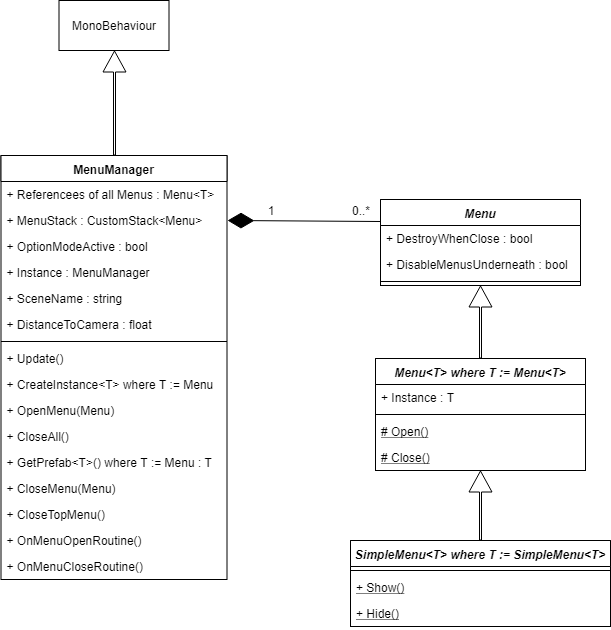
\includegraphics[width=11cm]{UI-System}
    \caption{Klassendiagramm des UI-Systems in C.LABEL-VR}
    \label{fig:UI-System}
\end{figure}

Der Ausgangspunkt des UI-Systems ist der \textit{MenuManager} (siehe Abbildung \ref{fig:UI-System}). Er bietet die Grundfunktionen, die notwendig sind um UI-Fenster zu öffnen, zu schließen und zu verwalten. Dazu besitzt er einen Stack der mit User Interfaces befüllt werden kann. Das oberste Element des Stacks ist dabei immer das, welches für den Benutzer sichtbar ist. Wird eine neues Fenster geöffnet, wird es oben auf den Stack gelegt und alle Elemente darunter werden deaktiviert, sofern dies für das neue Fenster so implementiert ist.\\

Die Elemente des Stacks sind dabei Klassen mit dem Namen \textit{Menu}. Dies ist die Basisklasse der UI-Elemente und beinhaltet zwei Bool-Werte, die besagen, ob das Fenster beim Schließen aus dem Speicher gelöscht wird (\textit{DestroyWhenClose}) und, ob alle Fenster, die im Stack unter dem jeweiligen Element sind, deaktiviert werden. Diese Basisklasse wird spezifiziert durch die Klasse \textit{Menu<T>}. Das Attribut \textit{<T>} einer Klasse deutet die Implementation einer generischen Klasse in C\# an. Diese Klassen kapseln Eigenschaften und Funktionen, die nicht für einen bestimmten Datentyp sind \cite{bib:Generics}. In Menu<T> steht das T für die Ausgangsklasse Menu<T>. Dies bewirkt, dass für T eine beliebige Klasse eingesetzt werden kann, solange diese von Menu<T> erbt, wobei T in diesem Fall für die beliebige Klasse steht. Das bedeutet, wenn beispielsweise eine Klasse \textit{TestUi} erstellt wird, welche von Menu<TestUi> erbt, ist dies eine valide Menu-Klasse und kann im Stack des MenuManagers aufgenommen werden. Auf diese Weise kann jedes Ui-Fenster, innerhalb der erstellten Klasse (z.B. TestUi),  mit individuellen Eigenschaften und Funktionen ausgestattet werden und trotzdem als allgemeines Menu-Element angesehen werden, welches vom MenuManager verwaltet werden kann. Die Klasse \textit{SimpleMenu<T>} ist eine Spezifikation der Klasse Menu<T> und ist für Benutzeroberflächen gedacht, die nur angezeigt und wieder geschlossen werden. Diese Klasse bietet nämlich nur die zwei Funktionen \textit{Show()} und \textit{Hide()}, um das Fenster simpel zu öffnen und zu schließen.\\

Das Aussehen der UI-Fenster und Anordnung der UI-Elemente, wie Buttons, Textfelder oder Eingabefelder, wird mit dem Unity Editor erstellt, der in Kapitel \ref{sec:UnityDevelopment} vorgestellt wurde. Um das erstellte Fenster mit dem vorgestellten UI-System benutzen zu können, muss es als Prefab abgespeichert sein. Diesem Prefab kann nun ein Skript zugewiesen werden, welches alle gewünschten Eigenschaften und Funktionalitäten des erstellten Fensters implementiert. Das Skript, beispielsweise mit dem Namen \textit{TestScript}, muss von der Klasse Menu<T> erben, also in diesem Fall von Menu<TestScript>. Ebenfalls muss das Skript im MenuManager referenziert sein (siehe \textit{References of Menus} in der Abbildung \ref{fig:UI-System}). Dadurch kann ein Entwickler, an einer beliebigen Stelle im Programm, ein UI-Fenster durch einen einzeiligen Aufruf öffnen (Zeile \ref{lst:OpenCall} in Auflistung \ref{lst:OpenMenu}). Durch die Referenzierung, die eben genannt wurde, kann der MenuManager das UI-Prefab, dem das Skript TestScript angehängt ist, instantiieren (Zeile \ref{lst:CreateInstance}) und anschließend den Öffnungsvorgang des Fensters, mit Hilfe der Instanz einleiten (Zeile \ref{lst:OpenInstance}). 

\begin{lstlisting}[caption={Aufruf und Implementierung der Funktion Open() einer Menu<T> Klasse}, captionpos=t, numbers=left,,escapeinside={(*@}{@*)}, label=lst:OpenMenu]
//Aufruf der Open()-Funktion eines Menu<T>-Klasse
TestScript.Instance.Open(); (*@ \label{lst:OpenCall} @*)

//Implementation der Open()
protected static void Open()
    {
        if (Instance == null)
		//T ist der Typ des aufrufenden Skripts, 
		//in diesem Fall also TestScript
            MenuManager.Instance.CreateInstance<T>(); (*@ \label{lst:CreateInstance} @*)
        else
            Instance.gameObject.SetActive(true);

        MenuManager.Instance.OpenMenu(Instance);(*@ \label{lst:OpenInstance} @*)
    }
\end{lstlisting}
\quad

\begin{figure}%
	\centering
    \fbox{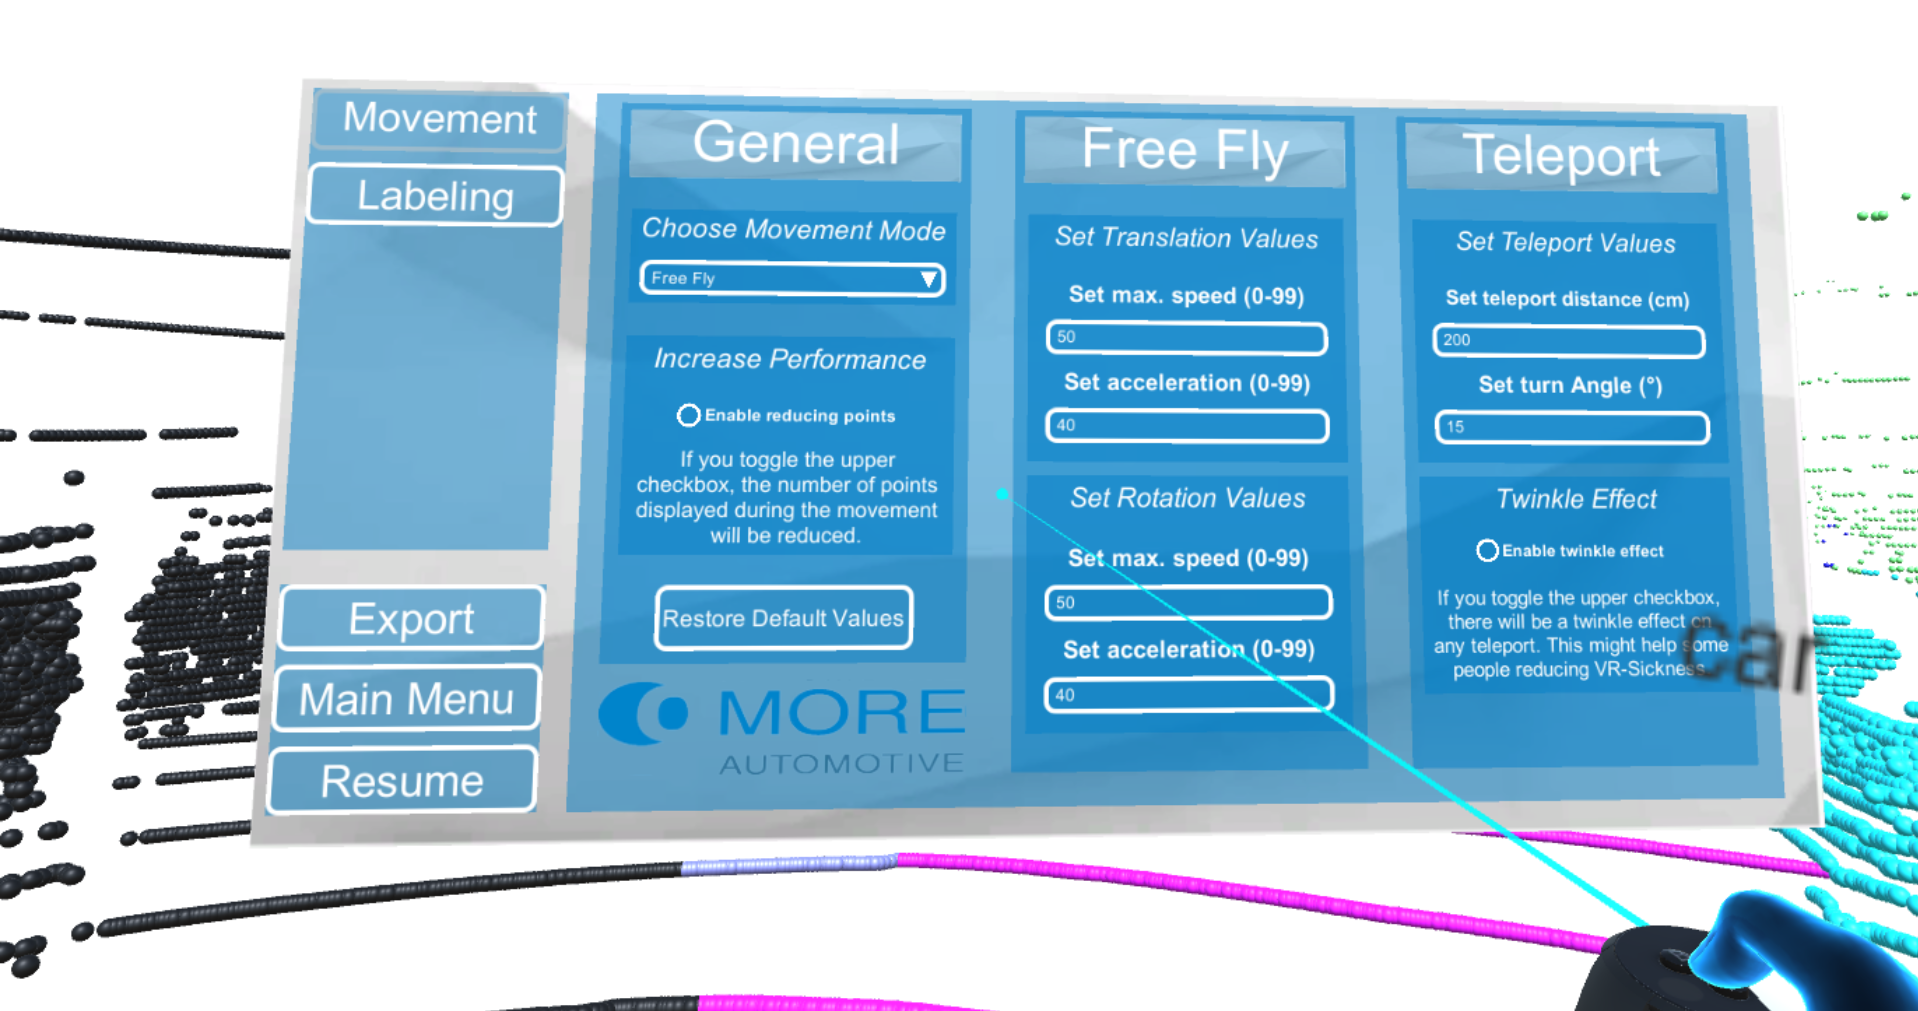
\includegraphics[width=15cm]{UiInSession}}
    \caption{Geöffnetes Applikationsmenü innerhalb einer Punktwolke}
    \label{fig:UiInSession}
\end{figure}

Der Öffnungsvorgang selbst, also die Funktion \textit{OpenMenu(Instance)}, legt die Instanz des UI-Fensters auf den Stack und macht alle Fenster, die sich darunter befinden unsichtbar, sofern dies vom Programmierer gewünscht ist (siehe \textit{DisableMenusUnderneith} in Abbildung \ref{fig:UI-System}). Anschließend wird die Sichtbarkeit des Fensters aktiviert. Bei normalen Desktop-Applikationen wäre der Öffnungsvorgang nun abgeschlossen, da Benutzeroberflächen auf einem Computermonitor nur eine zweidimensionale Position und Orientierung haben. In einer VR-Umgebung, ist jedes UI-Fenster aber eine dreidimensionale Komponente, die richtig im Raum platziert werden muss. Da sich der Benutzer stets bewegen und drehen kann, muss bei jedem Öffnungsvorgang eines UI-Fensters sichergestellt werden, dass das Fenster auch im Sichtfeld des Benutzers ist. Dazu wird innerhalb der OpenMenu(Instance)-Funktion die Position und Orientierung, der zu öffnenden Benutzeroberfläche, an die Position und Orientierung des Benutzers angepasst. Bei der Positionsanpassung muss beachtet werden, dass das Fenster nicht direkt an die Position des Benutzers gesetzt werden darf, sondern an einer Position vor dem Benutzer (siehe Abbildung \ref{fig:UiInSession}). Hierbei muss beachtet werden, dass der Abstand zum Benutzer abhängig von der Größe der Benutzeroberfläche ist. Ist diese beispielsweise klein und wird sehr weit vom Benutzer entfernt dargestellt, kann der Benutzer den Inhalt des Fensters nicht mehr richtig wahrnehmen. In C.LABEL-VR hat deshalb jedes UI-Fenster die selbe Größe, damit immer der gleiche Abstand benutzt werden kann.\\

Durch das vorgestellte UI-System können Funktionen und Eigenschaften von Benutzeroberflächen individuell gestaltet und trotzdem, vom Programmierer, simpel geöffnet und geschlossen werden. Durch die dynamische Anpassung der Position und Orientierung der UI-Fenster, kann das System auch in einer dreidimensionalen Umgebung, wie der virtuellen Realität, genutzt werden. So ist es möglich auch innerhalb einer Punktwolke Benutzeroberflächen aufzurufen. Die Funktionalitäten der Benutzeroberflächen, welche während einer Session in C.LABEL-VR aufgerufen werden können, sollen im folgenden Kapitel näher beschrieben werden.
  
\subsection{Applikations-Menü}
\label{sec:AppMenu}
\begin{figure}
    \centering
    \subfloat[Bewegungsmenü]{{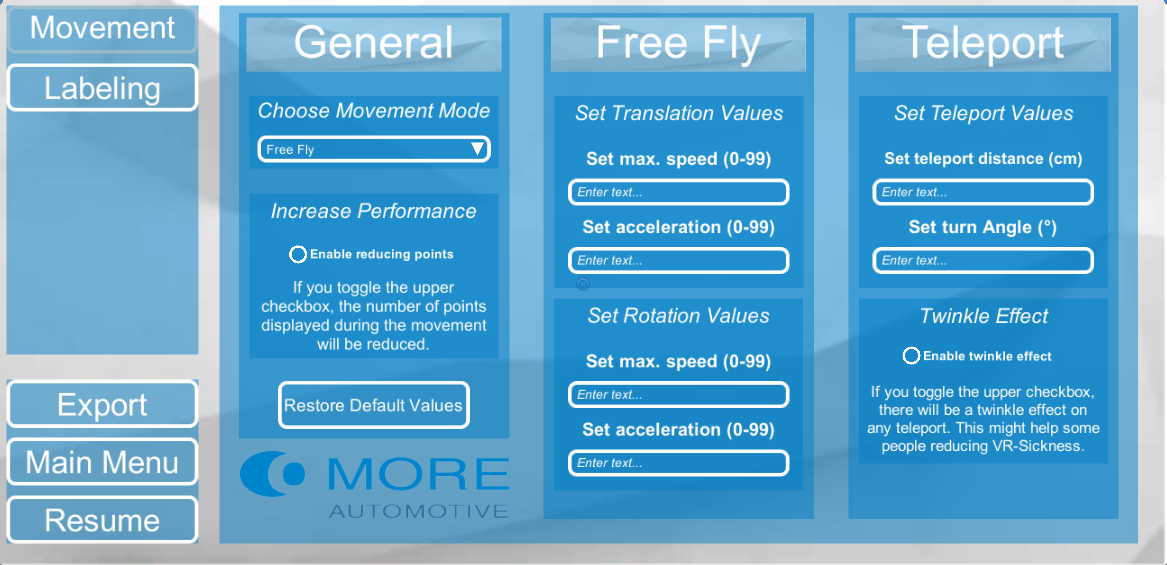
\includegraphics[width=14cm]{MovementMenu}\label{fig:MovementMenu}}}%
    \qquad
    \subfloat[Klassifikationsmenü]{{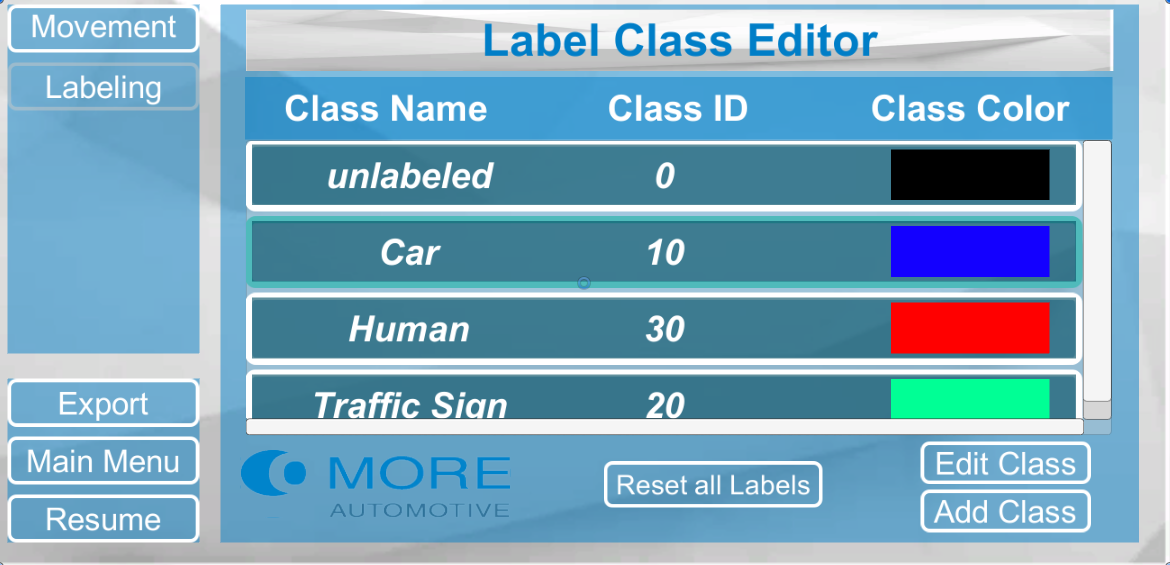
\includegraphics[width=14cm]{LabelingMenu}\label{fig:LabelingMenu}}}%
    \caption{Die Abbildungen zeigen die zwei Benutzeroberflächen, die innerhalb einer Session in C.LABEL-VR aufgerufen werden können.}\label{fig:ApplicationMenu}%
\end{figure}

Innerhalb einer Session gibt es ein Applikationsmenü, welches der Benutzer aufrufen kann. Dieses enthält zwei Benutzeroberflächen. Zum einen gibt es eine Benutzeroberfläche zur Anpassung von Bewegungsparametern. Zum Anderen gibt es ein Fenster zum editieren und erstellen von Klassifikationen, welche innerhalb der Session zum Labeln von Punkten verwendet werden können. Das Applikationsmenü wird mit Hilfe des UI-System geöffnet und geschlossen, welches im vorherigen Abschnitt \ref{sec:UIMenu} vorgestellt wurde. Das Menü erscheint also stets in der richtigen Orientierung im Sichtfeld des Benutzers.\\

\subsubsection{Bewegungsmenü}

Das Menü zur Einstellung von Bewegungsparametern, im Folgenden Bewegungsmenü genannt, bietet sowohl allgemeine, als auch spezifische Parameter für die einzelnen Navigationsarten (siehe Abbildung \ref{fig:MovementMenu}). Im der Sektion \textit{General} sind die allgemeinen Einstellungsmöglichkeiten zu finden. Hier kann zum einen die Navigationsart festgelegt werden (\textit{Choose Movement Mode}) und zum anderen können alle Bewegungsparameter auf die Ausgangswerte gesetzt werden (\textit{Restore Default Values}). Des Weiteren gibt es eine  Einstellung zur Verbesserung der Bildwiederholungsrate, welche von der Bewegung des Benutzers abhängt. Wie schon in Kapitel \ref{sec:Optimierung} beschrieben, kann es bei zu vielen Punkten im Sichtfeld des Benutzers, zu einem Einbruch der Bildwiederholungsrate kommen. In diesem Fall kann das Markierungsfeld \textit{Enable reducing points} aktiviert werden. Auf diese Weise werden die angezeigten Punkte einer Punktwolke reduziert, solange sich der Benutzer bewegt. Sobald der Benutzer aufhört sich zu bewegen, werden wieder alle Punkte visualisiert. Somit kann eine hohe Bildwiederholungsrate während der Bewegung auch dann sichergestellt werden, wenn sich zu viele Objekte im Sichtfeld des Benutzers befinden.\\

In der Sektion \textit{FreeFly} kann der Benutzer Einstellungen im Bezug auf den freien Flugmodus (siehe Kapitel \ref{sec:FreeFlyMode}) vornehmen. Die Bewegung innerhalb des freien Flugmodus basiert auf konstanter Bewegung mit einer Maximalgeschwindigkeit. Die Maximalgeschwindigkeit wird dabei nach einer gewissen Beschleunigungsphase erreicht. Sowohl die Maximalgeschwindigkeit, als auch die Beschleunigung wird dabei mit einem Faktor multipliziert. Diesen Faktor kann der Benutzer im Bewegungsmenü selbst festlegen. Diese Möglichkeit besteht für die Bewegung in Translatorischer Form und für die Rotation um die eigene Achse des Benutzers. Somit kann sich der Benutzer die eigene Positions- und Orientierungsveränderung individuell einstellen. Nutzer, bei denen beispielsweise keine Symptome der VR-Krankheit auftreten, können sich somit schnell durch die Punktwolke bewegen. Nutzer, bei denen die Symptome auftreten, können sich langsamer bewegen um die Symptome gering zu halten.\\

In der Sektion \textit{Teleport} kann der Benutzer Einstellungen im Bezug auf den Teleport-Modus (siehe Kapitel \ref{sec:TeleportMode}) vornehmen. Bei diesem Modus werden die Symptome der VR-Krankheit verhindert, indem die Bewegung des Benutzers durch sofortige und einmalige Positions- und Orientierungsveränderung erfolgt. Auf diese Weise wird der Benutzer, für jeden Bewegungsbefehl, um eine gewisse Distanz verschoben, oder um einen gewissen Winkel gedreht. Die Verschiebungsdistanz und der Drehwinkel kann vom Benutzer selbst im Bewegungsmenü eingestellt werden. Des Weiteren gibt es die Möglichkeit, innerhalb des Teleport-Modus, einen Zwinker-Effekt bei jeder Bewegung und Drehung auszulösen. Dazu muss das Markierungsfeld \textit{Enable twinkle effect} aktiviert sein. Die Simulation eines Augenzwinkerns soll ebenfalls die Symptome der VR-Krankheit verhindern. TODO TEXT quelle.\\


\subsubsection{Bewegungsmenü}

\begin{figure}%
	\centering
    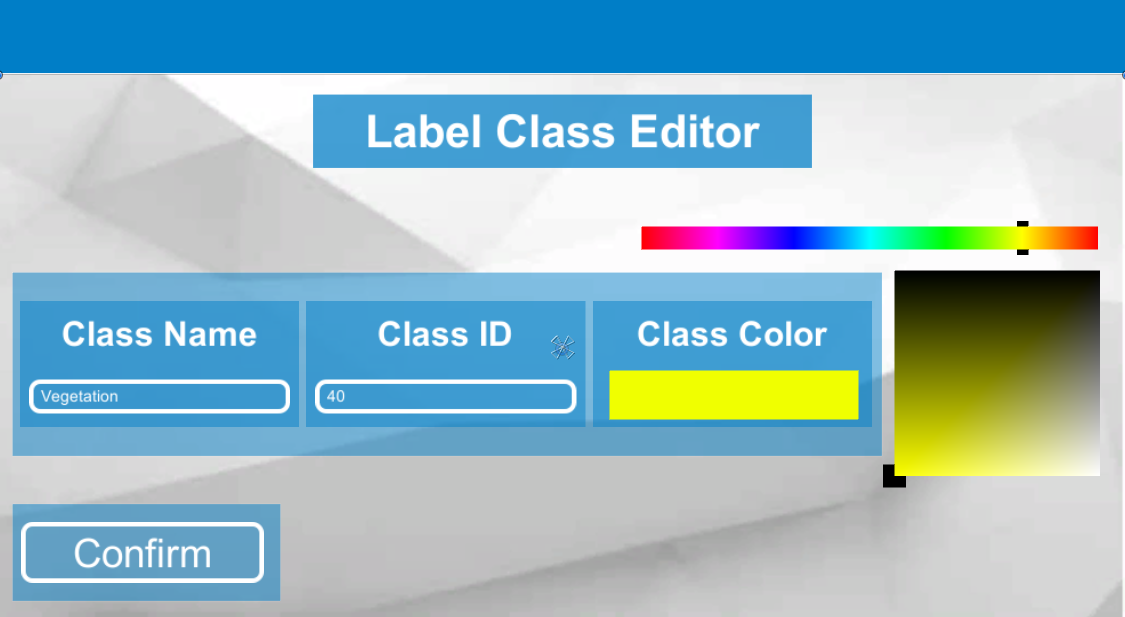
\includegraphics[width=11cm]{LabelClassEditor}
    \caption{Benutzeroberfläche zum erstellen oder editieren einer Klassifikation}
    \label{fig:LabelClassEditor}
\end{figure}
Im zweiten Applikationsmenü können Einstellungen im Bezug auf die Klassifikationen innerhalb einer Session vorgenommen werden (siehe Abbildung \ref{fig:LabelingMenu}). Innerhalb dieser Benutzeroberfläche werden alle Klassifikationen mit Name und der jeweiligen ID und Farbe dargestellt, die aktuell in der Session vorhanden sind. Die Farbe repräsentiert dabei die Farbe, mit der die Punkte in der Punktwolke dargestellt werden, welche mit der jeweiligen Klassifikation versehen sind. Alle Punkte mit dem Label \textit{Car} sind demnach in blau dargestellt (vgl. Klassifikation Car in Abbildun \ref{fig:LabelingMenu}). Der Benutzer hat innerhalb dieses UI-Fensters die Möglichkeit neue Klassifikationen zu erstellen. Durch Betätigung des Knopfes \textit{Add Class} öffnet sich ein neues UI-Element, mit dem Name, ID und die Farbe der neuen Klassifikation angegeben werden können (siehe Abbildung \ref{fig:LabelClassEditor}). 

Darüber hinaus können alle aktuell verfügbaren Klassifikationen vom Benutzer verändert werden. Dazu wird die gewünschte Klassifikation ausgewählt und danach der Knopf \textit{Edit Class} betätigt. In der Abbildung (siehe Abbildung \ref{fig:LabelingMenu}) ist die Klasse Car markiert, was durch den farbigen Rand signalisiert ist. Durch die Betätigung des Edit Class-Knopfes öffnet sich das gleiche UI-Fenster wie beim erstellen einer neuen Klasse, mit dem Unterschied, dass nun die Felder für Namen, ID und Farbe schon einen Wert haben. Nach der gewünschten Änderung der Klassifikation werden alle Änderungen auf diejenigen Punkte in der Punktwolke wirksam, welche dieses Label bereits besitzen. 

Des weiteren gibt es die Möglichkeit durch Betätigung des Knopfes \textit{Reset all Labels} alle Klassifikationen der Punkte zu löschen. Auf diese Weise werden alle Punkte mit der Klassifikation \textit{unlabeled} versehen. Diese Funktion ist gerade bei Demonstrationszwecken der Applikation notwendig, damit jedem Probanden schnell, eine ungelabelte Punktwolke zur Verfügung gestellt werden kann. 